%% 
%% Copyright 2007, 2008, 2009 Elsevier Ltd
%% 
%% This file is part of the 'Elsarticle Bundle'.
%% ---------------------------------------------
%% 
%% It may be distributed under the conditions of the LaTeX Project Public
%% License, either version 1.2 of this license or (at your option) any
%% later version.  The latest version of this license is in
%%    http://www.latex-project.org/lppl.txt
%% and version 1.2 or later is part of all distributions of LaTeX
%% version 1999/12/01 or later.
%% 
%% The list of all files belonging to the 'Elsarticle Bundle' is
%% given in the file `manifest.txt'.
%% 

%% Template article for Elsevier's document class `elsarticle'
%% with numbered style bibliographic references
%% SP 2008/03/01

\documentclass[preprint,12pt]{elsarticle} %elsarticle

\usepackage[T1]{fontenc}
\usepackage[utf8]{inputenc} %latin1
\usepackage{amsmath,amssymb}
\usepackage{url}
\usepackage{graphicx}
\usepackage[caption=false]{subfig}
\usepackage{braket}
\usepackage{amsfonts}
\usepackage{amsthm}
\usepackage{fancyhdr}
\usepackage{comment}
\usepackage{float}
\usepackage{mathtools}
\usepackage{xspace}
\usepackage[inline]{enumitem}
\usepackage[export]{adjustbox}
\usepackage[numbers]{natbib}
\bibliographystyle{IEEEtranN}


 %\usepackage{subfigure}
%\usepackage{subcaption}
%\usepackage[subfigure]{tocloft}
%\usepackage[subfigure]{tocloft} 
%\usepackage{subfigure} 
\usepackage{marginnote}
\usepackage[usenames, dvipsnames]{color}
\usepackage[nameinlink, nosort]{cleveref}
\usepackage{lscape} %folha em paisagem
%\usepackage[alf]{abntex2cite} %Included by me
%\bibliographystyle{abntex2-alf}
%\usepackage[square]{natbib}
% \usepackage{indentfirst}

% \title{The Complexity of $B_{1}$-EPG-Helly Graph Recognition} 

\newtheorem{theorem}{Theorem}
\newtheorem{lema}[theorem]{Lemma}
\newtheorem{defi}[theorem]{Definition}
\newtheorem{coro}[theorem]{Corollary}
\newtheorem{prop}[theorem]{Proposition}
\newtheorem{fact}[theorem]{Fact}
\renewcommand{\proofname}{Proof}

\newcommand\floor[1]{\left\lfloor #1 \right\rfloor}
\newcommand\toricclass[1]{#1_\circ^\circ}
\newcommand{\toric}[1]{\left[#1\right]^\circ_\circ}
\renewcommand\mod[1]{\!\!\!\!\!\pmod{#1}}

%\hyphenation{re-pre-sen-ta-ção}


%% Use the option review to obtain double line spacing
%% \documentclass[authoryear,preprint,review,12pt]{elsarticle}

%% Use the options 1p,twocolumn; 3p; 3p,twocolumn; 5p; or 5p,twocolumn
%% for a journal layout:
%% \documentclass[final,1p,times]{elsarticle}
%% \documentclass[final,1p,times,twocolumn]{elsarticle}
%% \documentclass[final,3p,times]{elsarticle}
%% \documentclass[final,3p,times,twocolumn]{elsarticle}
%% \documentclass[final,5p,times]{elsarticle}
%% \documentclass[final,5p,times,twocolumn]{elsarticle}

%% For including figures, graphicx.sty has been loaded in
%% elsarticle.cls. If you prefer to use the old commands
%% please give \usepackage{epsfig}

%% The amssymb package provides various useful mathematical symbols
%\usepackage{amssymb}
%% The amsthm package provides extended theorem environments
%% \usepackage{amsthm}

%% The lineno packages adds line numbers. Start line numbering with
%% \begin{linenumbers}, end it with \end{linenumbers}. Or switch it on
%% for the whole article with \linenumbers.
%% \usepackage{lineno}

\journal{Information Processing Letters}

\begin{document}

\begin{frontmatter}

%% Title, authors and addresses

%% use the tnoteref command within \title for footnotes;
%% use the tnotetext command for theassociated footnote;
%% use the fnref command within \author or \address for footnotes;
%% use the fntext command for theassociated footnote;
%% use the corref command within \author for corresponding author footnotes;
%% use the cortext command for theassociated footnote;
%% use the ead command for the email address,
%% and the form \ead[url] for the home page:
%% \title{Title\tnoteref{label1}}
%% \tnotetext[label1]{}
%% \author{Name\corref{cor1}\fnref{label2}}
%% \ead{email address}
%% \ead[url]{home page}
%% \fntext[label2]{}
%% \cortext[cor1]{}
%% \address{Address\fnref{label3}}
%% \fntext[label3]{}

\title{The Complexity of $B_{1}$-EPG-Helly Graph Recognition}

%% use optional labels to link authors explicitly to addresses:
%% \author[label1,label2]{}
%% \address[label1]{}
%% \address[label2]{}

\author{Claudson Bornstein$^{1}$, Martin C. Golumbic$^{2}$, \\Tanilson Santos$^{1,3}$, Uéverton Souza$^{4}$, Jayme Szwarcfiter$^{1,5}$
}

\address{$^{1}$Federal University of Rio de Janeiro - Brazil, 
\\$^{2}$University of Haifa - Israel,
\\$^{3}$Federal University of Tocantins  - Brazil, \\$^{4}$Fluminense Federal University - Brazil, \\$^{5}$State University of Rio de Janeiro - Brazil}

% \address{$^{1}$Universidade Federal do Rio de Janeiro - UFRJ, \\$^{2}$Universidade Federal do Tocantins - UFT, \\$^{3}$Universidade Federal do Fluminense - UFF, \\$^{4}$Universidade do Estado do Rio de Janeiro - UERJ}


\begin{abstract}
Golumbic, Lipshteyn and Stern defined in 2009 the class of EPG graphs, an intersection graph class  based on edge intersection of paths on a grid. An EPG graph $G$ is a graph that admits a representation where its vertices correspond to paths in a grid $Q$, such that two vertices of $G$ are adjacent if and only if their corresponding paths in $Q$ have a common edge. If the paths in the representation have at most $k$ changes of direction  (bends), we say that this is a  $B_k$-EPG representation. A collection $C$ of sets satisfies the Helly property when every sub-collection of $C$ that is pairwise intersecting has at least a common element. In this paper we show that the problem of recognizing $B_1$-EPG graphs whose edge-intersections of paths in a grid satisfy the Helly property is NP-complete.  
\end{abstract}

\begin{keyword}
%% keywords here, in the form: keyword \sep keyword
EPG \sep Intersection Graphs\sep Helly\sep Single Bend\sep NP-completeness.
%% PACS codes here, in the form: \PACS code \sep code

%% MSC codes here, in the form: \MSC code \sep code
%% or \MSC[2008] code \sep code (2000 is the default)

\end{keyword}

\end{frontmatter}

% \linenumbers

\section{Introduction}

An EPG graph $G$ is a graph that admits a representation in which its vertices are represented by paths of a grid $Q$, such that two vertices of $G$ are adjacent if and only the corresponding paths having at least one common edge. The study of EPG graphs has some practical motivations. For example, it is related to the problem of layout of digital circuits, which can be represented as paths in a rectangular orthogonal grid.

%Every graph $G$ has an EPG representation, see~\citep{golumbic2009}. 
A graph is a $ B_k$-EPG graph if it admits a representation of this graph in which each path has at most $k$ bends. As an example, Figure~\ref{fig:trianguloepgRepresentacao}(a) shows a $C_3$, Figure~\ref{fig:trianguloepgRepresentacao}(b) shows an EPG representation where the paths have no bends, Figure~\ref{fig:trianguloepgRepresentacao}(c) shows a representation with 1 bend, and Figure~~\ref{fig:trianguloepgRepresentacao}(d) shows a representation where every path has at most 2 bends. Consequently, $C_3$ is a $B_0$-EPG graph. More generally, $B_0$-EPG graphs coincide with interval graphs.

For some classes of graphs we know the smallest value of $k$ for which the graphs in the class are $B_k$-EPG. For example, interval graphs are $B_0$-EPG, trees are contained in $ B_1$-EPG, outerplanar graphs are contained in $B_2$-EPG, and planar graphs are contained in $ B_4 $-EPG. Although no example has yet been found of a planar graph that fails to be B3-EPG.
% although no example has yet been found of a planar graph that fails to be B3-EPG

The class of EPG graphs has been studied in several papers, such as \citep{golumbic2009, alcon2016, cohen2014, Asinowski2009, martin2017, heldt2014}, among others. The investigations frequently approach characterizations with respect to the number of bends of the graph representation. Regarding the complexity of recognition of $B_k$-EPG graphs, only the complexity of recognizing three of these sub-classes of EPG graphs have been determined: $ B_0$-EPG, $ B_1$-EPG ~\citep{heldt2014} and more recently $B_2$-EPG ~\citep {martin2017}.  $ B_0$-EPG graphs can be recognized in polynomial time, since it corresponds to the class of interval graphs, see ~\citep{booth1976}. 

\begin{figure}[h]
  \centering
  \begin{tabular}{ p{6cm} p{6cm} }
    \centering 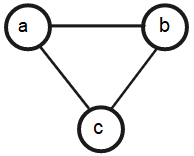
\includegraphics[width=2.3cm]{./img/trianguloabc.png} & 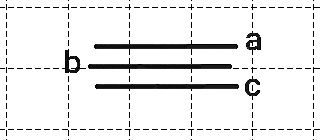
\includegraphics[width=3.5cm]{./img/b0epgTransparenciaGrade2.png}
    \\
    \footnotesize \centering (a) The  graph $C_3$ & \footnotesize(b) $B_0$-EPG representation of $C_3$  \\
&  \\ \centering
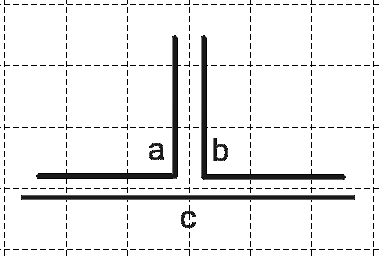
\includegraphics[width=3.5cm]{./img/b1EpgTransparenteGrade2.png} %b1epgtriangulo
     & 
  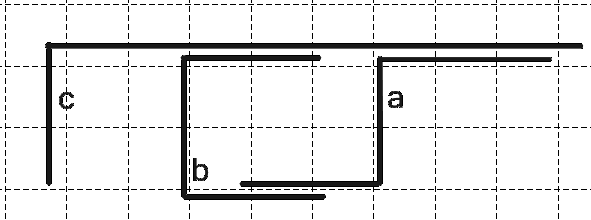
\includegraphics[width=5cm]{./img/b2epgTransparenciaGrade2.png}\\
  \footnotesize \centering (c) $B_1$-EPG representation of $C_3$  &  \footnotesize  (d) $B_2$-EPG representation of $C_3$ \\
  \end{tabular}

 \caption{The  graph $ C_3 $  and some representations: without bends, with 1 bend and with 2 bends} \label{fig:trianguloepgRepresentacao}
\end{figure}


%A  collection $C$ of sets satisfies the Helly property when every sub-collection of $ C $ that is pairwise intersecting has at least one common element. The Helly property has this name in honor of the great Austrian mathematician Eduard Helly, who in 1923 proposed his famous theorem concerning the relation of intersecting sets.

%The study of the Helly property is useful in very diverse areas of science, and we can enumerate applications in semantics, code theory, computational biology, database, image processing, graph theory, optimization, and linear programming \citep{dourado2009}.

%Note that the representation of Figure~\ref{fig:trianguloepgRepresentacao}(b) satisfies the Helly property, while the representations of Figures~\ref{fig:trianguloepgRepresentacao}(c) and~\ref{fig:trianguloepgRepresentacao}(d) do not satisfy it.


This paper studies graphs that have an EPG-Helly representation. We prove that the problem of recognizing $ B_1$-EPG-Helly graphs is $NP$-complete.  So far, the only papers that have approached the Helly property related to EPG representations of graphs are \cite{golumbic2009} and \cite{golumbic2013}. In particular, the graphs they have studied $B_1$-EPG representations. 

% recognition problem.% whose representation has the Helly property.

   %@comment retirado para o SBPO
   %Dessa forma, para situar o leitor neste contexto, são definidos na seção seguinte os principais termos utilizados ao longo deste escrito. 
 
 
 %\subsection{Basic definitions}
 Next, we describe some terminology and notation employed.

%@comment falar q a diagonal não é considerada
%ver se o conceito de direção não confunde com caminho direcionado

The term \emph{grid} is used to denote the Euclidean space of integer orthogonal coordinates. Each pair of integers are the \emph{coordinates} of a point in the grid, when convenient we will call it as a \emph {vertex of the grid}. The term \emph{edge of the grid}, will be used to denote a pair of vertices that are at a distance one in the grid. Two edges $e_1$ and $e_2$ are \emph{consecutive edges} when they share exactly one coordinate of the grid. %have a common vertex. %A \emph{finite sequence of consecutive edges} is a finite sequence where every vertices are differents  
 A \emph{path in the grid} is any finite sequence of consecutive edges, without edge repetition, of the grid. The first and last edges of a path are called \emph{extremity edges}.
The \emph{direction of an edge} is vertical when the first coordinate of its vertices  are equal, and is horizontal when the second coordinates are equal. A \emph {bend} in a path is a pair of consecutive edges $ e_1, e_2 $ of that path, such that the directions of $ e_1$ and $ e_2$ are different. When two edges $ e_1$ and $e_2 $ form a bend, they are called \emph { bend edges}. A \emph {grid segment} is a set of consecutive edges with no bends. %is a path with no bends.
 Two paths are said to be \emph{edge-intersecting}, or  simply  \emph{intersecting}, if they share at least one edge. %Otherwise we say they are \emph{edge-disjoint} (or disjoint).
 Through the paper any time we say that two paths intersect, we mean they edge-intersect.  %, all intersections of paths are meant to edge intersections.

By EPG graphs, we denote the class of intersection graphs of paths in a grid. This class, defined in 2009~\citep{golumbic2009}, consists of the class of graphs in which its vertices are represented by paths of a grid $ Q $, such that two vertices in $ G $ are adjacent if and only if their corresponding paths in $ Q $ intersect. If every path in a representation can be represented with at most $ k $ bends, we say that this graph $ G $ has a \emph{ $ B_k$-EPG} representation.%, and we will indicate this representation by the notation $ B_k$-EPG($ G $).
When $ k = 1 $ we say that this is a \emph{single bend} representation.


%Two sets, $ A $ and $ B $, are \emph{intersecting} $ A \cap B \neq \emptyset $. 
A family of sets is said to be \emph{pairwise intersecting} if any two sets in the family intersect. A collection of non-empty sets $C$ satisfies the Helly property when every pairwise intersecting sub-collection of $ C $ has one element that is in every subset of $C$.

The Helly property can be applied to the $ B_k $-EPG representation problem, where each path is considered a set of edges. A graph $ G $ has a  $ B_k$-EPG-Helly representation if there is a $ B_k $-EPG representation of $G$ where each path has at most $ k $ bends and this representation satisfies the Helly property. %Further for all subset of pairwise intersecting paths, there is an edge common to all paths of this subset, we will indicate this representation by the notation H-$B_k$-EPG($G$). 
 Figure~\ref{fig:envelopeRepresentacoes}(a) presents two $B_1$-EPG representations of a graph with five vertices.  Figure~\ref{fig:envelopeRepresentacoes}(b)   presents 3 pairwise intersecting paths ($p(v_1), p(v_2), p(v_5)$), containing a common edge to the paths, so it is a valid $ B_1$-EPG-Helly representation. In Figure~\ref{fig:envelopeRepresentacoes}(c), although the three paths are pairwise intersecting, there is no common edge in all 3 paths, and therefore they do not satisfy the Helly property. 

\begin{figure}[h]
  \centering
  \begin{tabular}{ p{6cm} c p{6cm} }
    \centering 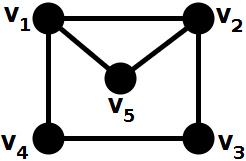
\includegraphics[width=4cm]{./img/envelope.png} & & 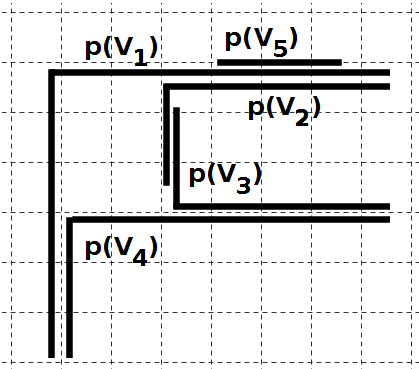
\includegraphics[width=5cm]{./img/envelopeHellyGradeTransparente.png}
    \\
    \footnotesize \centering (a) A  graph with 5 vertices && \footnotesize(b) $B_1$-EPG representation that satisfies the Helly property  \\
&&  \\ 

\begin{tabular}[c]{@{}l@{}} 
\hspace{3.3cm} 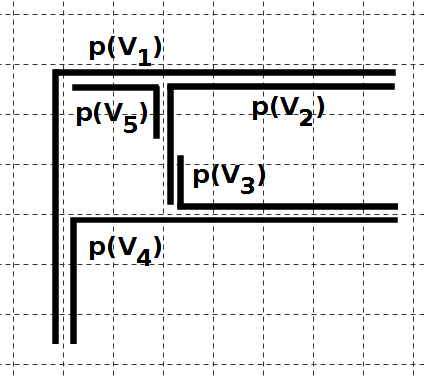
\includegraphics[width=5.5cm]{./img/envelopeNaoHellyGrade.png} %b1epgtriangulo
\\
 \hspace{3.3cm} \footnotesize (c) $B_1$-EPG representation that does\\ 
 \hspace{3.3cm} \footnotesize not satisfy the Helly property
\end{tabular}

% \centering &
% 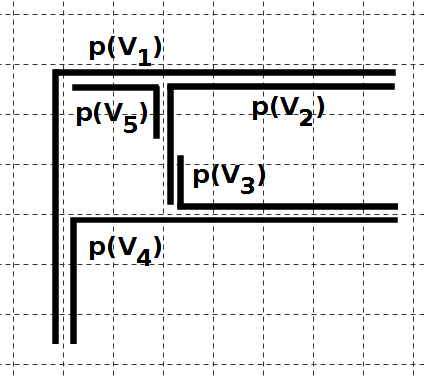
\includegraphics[width=5cm]{./img/envelopeNaoHellyGrade.png} %b1epgtriangulo
%       &
%  \\
%   \footnotesize \centering (c) $B_1$-EPG representation that not satisfies the Helly property &  &  \\
  \end{tabular}

 \caption{A  graph with 5 vertices in (a) and some single bend representations: Helly in (b) and not Helly in (c)} \label{fig:envelopeRepresentacoes}
\end{figure}

%An \emph{edge (of the grid) is relevant} if at least one of its coordinates is the start, bend, or end of a path. A  \emph{maximal segment} is one whose its ends are relevant edges.  

%A $B_k$-EPG representation \emph{is normalized} when all columns $(i,i+1)$ and lines $(j,j+1)$ that have only not relevant edges in the representation have been removed. 

 The next lemma, shows that every graph is an EPG-graph.
 
 \begin{lema} \citep{golumbic2009} \label{lem:todoGrafoEpg}
 Every graph is an EPG graph.
 \end{lema}
%  \begin{proof}
%  Let $G=(V,E)$ be a graph with vertices $v_1,\dots ,v_n$. Consider the grid $Q$ with rows $[1,\dots ,n]$ and columns $[1, 1', 2, 2', \dots, n,n']$. 
 
%  Consider the vertex $v_i$ and denote $N^+(v_i)$= $\{v_j|i<j,(i,j)\in E\}$, where $N^+(v_i)$= $\{v_{j_1}, \dots, v_{j_k}\}$ is ordered with $\{v_{j_1}< \dots < v_{j_k}\}$.   The path $P_i$ on $Q$ is defined starting horizontally from grid point $(1,i)$ to $(i,i)$, continuing vertically to $(i,j_1)$, horizontally to $(i',j_1)$, continuing vertically to $(i,j_2)$, horizontally to $(i',j_2)$, continuing vertically $(i,j_3)$, horizontally $(i',j_3)$, etc. i.e., we alternate between column $i$ and column $i'$ as we go across on each level $j_1, j_2, \dots, j_k$. %reference Figure
%  We prove that $P_i$ on the grid $Q$ is an EPG representation of $G$. For every $i<j,(v_i,v_j)\in E(G)$ if and only if the paths $P_i$, $P_j$ contain the horizontal grid edge $((i,j), (i',j))$. Moreover, no paths share vertical grid edges. Therefore the vertices in the graph are adjacent if and only if the corresponding paths share a common grid edge.
%  \end{proof}
 
 Moreover, the same applies to EPG-Helly graphs. 
 
 \begin{lema}\label{lem:todoGrafoEpgHelly}
 Every graph is an EPG-Helly graph.
 \end{lema}
  \begin{proof}
  Let $G$ be a graph with $n$ vertices $v_1, v_2, \dots, v_n$ and $\mu$ maximal cliques $C_1, C_2, \dots , C_{\mu }$. We construct an EPG-Helly representation of $G$, using a grid $Q$ of size $(\mu \times 2n)$. The lines correspond to the maximal cliques and are numbered $1, 2, \dots , \mu$. Each vertex $v_j$ corresponds to the pair of columns $j, j+n$. Each maximal clique $C_i$ is mapped into an edge $(i,n), (i,n+1)$. Each path $P_j$ contains all edges $(i,n), (i,n+1)$ corresponding to the maximal cliques $C_i$ containing $v_i$.
  
  Moreover, two distinct paths $P_j,P_k$ intersect at the edges corresponding to the maximal cliques containing $v_j,v_k$.
  
  Let $v_j \in V(G)$, consider the maximal cliques containing $v_j$ in ascending order of their indices. The path $P_j$ representing $v_j$, start at vertex $(1,j)$ of $Q$ and descends column $j$ until $(i,j)$, where $C_i$ is the first clique containing $v_j$ then $P_j$ bends at vertex $(i,j)$ and proceeds to the right, travesses edge $(i,n), (i,n+1)$ representing $C_i$. Then $P_j$ proceeds further on line $i$ until reaching vertex $(i, j+n)$, where it bends again, descending column $j+n$ until reaching vertex $(l,j), l>i$, where $C_l$ is the next maximal clique containing $v_j$ where it bends again. It proceeds in line $l$, travessing edge $(l,n),(l,n+1)$, and so on, until all edges of $Q$ corresponding to the maximal cliques containing $v_j$ have been travessed by $P_j$.   
  
It follows that two distinct paths, $P_j$ and $P_q$, intersect exactly at the lines corresponding to the maximal cliques containing both $v_j$ and $v_q$.  
  
  
 %%%%%%%%%%%%%%%%%%%%%%
%  Take a grid $Q$ of dimension $(\mu \times 2n)$ such that the lines are numbered from $1$ to $ \mu$ (from top to bottom), where $\mu$ is the number of maximal cliques of the graph $G$, and the columns are numbered from $-n$ to $ -1$ and continuing from $1$ to $ n$ (from left to right). %Let $v_i, i = 1, \dots, n$ be vertices of $G$. 
%  Associate the $\mu$ maximal cliques in $\mu$ edges of the column $(-1, 1)$, such that the clique $C_1$ is represented by the first row from the top, the clique $C_2$ is represented by the second row, etc.  %and %so successively until the clique $c_\mu$ is on the last line bottom. 
%  For each path $P_i$ in each clique $C_j$ from the top to the bottom, do as follows: if $P_i$ occurs in only one clique then the segment $P_i$ is put in its place, in the edge associates to clique $C_j$, and is done; if $P_i$ occurs in more than one clique, the path $P_i$ elongates to the column $i$, it performs bend and continue to the point $(x,i)$ where there is a clique $C_x$  of which $P_i$ is part, so $P_i$ performs bend again and go to the point $(x,-i)$. If $P_i$ yet appears in another clique then  $P_i$ performs bend in $(x,-i)$, it continues until the next clique $C_y$ that $P_i$ is part. In point $(y,-i)$ the path performs bend again and go to the point $(y,i)$. 
%  The process is  repeated until every cliques that $P_i$ is part are covered. 
 
 
% Since all edges of the graph belong to some click of a click cover then this ensures that all edges are represented by the algorithm. As lines of the column  $ i $ and $ -i $ are dedicated only to the path $ P_i $ this ensures that intersections occur only in the horizontal direction, and the paths that intersect in the horizontal direction are only those that participate of the same click $ C_j $, so non-edges of the representation are also represented. Also, since all paths intersecting in the horizontal direction have to pass through the edge $ (- 1, 1) $ of a certain click $ C_j $ then they have at least one common edge, this ensures that the representation is Helly.
 \end{proof}
 
 Figure~\ref{fig:gradeDemonstracao} shows the grid $Q$ and the path $P_2$ corresponding to the vertex $v_2 \in V(G)$, contained in maximal cliques $C_2, C_4$ and $C_5$ of $G$.
 
  \begin{figure}[htb]	
\center%6.3
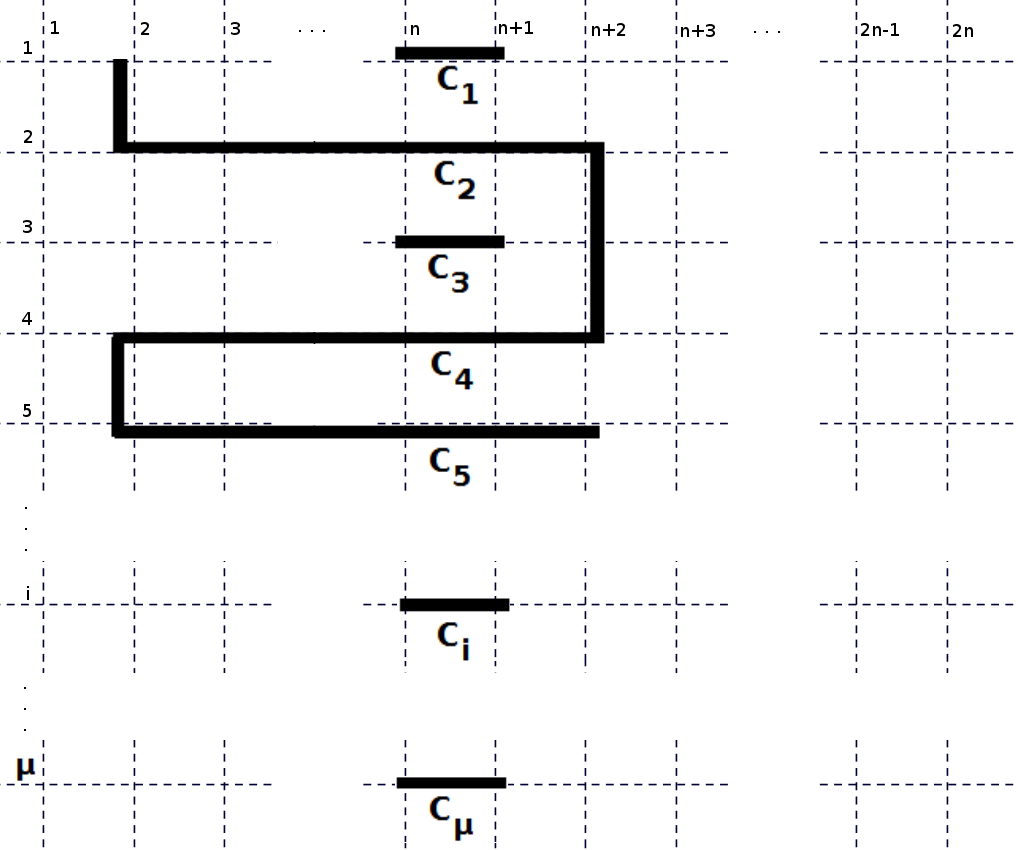
\includegraphics[width=10cm]{./img/grade2.png}
%clausulaGadgetGFCompletaSBPO
\caption{Representation of the path $P_2$ corresponding to vertex $v_2$ contained in cliques $C_2, C_4$ and $C_5$}
\label{fig:gradeDemonstracao}
\end{figure}
 
 
 \begin{coro}
 Every graph $G$ containing $\mu$ maximal cliques admits a $B_{2\mu -1}$-EPG-Helly representation. %in a grid $Q$ of dimension $(\mu \times 2n)$.
 \end{coro}
 
\section{Basic EPG representations}
%{The Classes $B_1$-EPG and $B_1$-EPG-Helly}

% Although classes $B_1$-EPG and $ B_1$-EPG-Helly do not coincide, see Lemma~\ref{lem:octaedronaohelly}, the same does not occur for classes $ B_0$-EPG and $ B_0$-EPG-Helly, as observed in Lemma~\ref{lem:b0epg}.

% \begin {lema} \label{lem:b0epg}
% Every $ B_0$-EPG representation satisfies the Helly property.
% \end {lema}
% \begin {proof}
% Assume by contradiction that there exists a graph $G$ that admits a $ B_0$-EPG representation that does not satisfy the Helly property. Then, this representation has a minimal collection $ P = \{p (v_1), p (v_2), \ldots, p (v_k) \} $ of mutually intersecting paths such that $$ p(v_1) \cap p(v_2 ) \cap \cdots \cap p(v_k) = \emptyset, k \geq 3. $$
% By minimality, we know that $ \bar{P_1} = P \setminus \{p (v_1) \}$, $ \bar {P_2} = P \setminus \{p(v_2) \} $ and $ \bar {P_3 } = P \setminus \{p (v_3) \} $ are mutually intersecting and satisfy the Helly property.
% Thus, there are the following distinct segments $ s_{\bar{P_1}}, s_{\bar {P_2}}, s_{\bar {P_3}}$ associated with the intersection of the paths in $ \bar {P_1},  \bar {P_2} $ and $ \bar {P_3} $. Since the representation has no paths with bends, then we know that the paths in $ P$ are on the same line.
% Without loss of generality, we can assume that $ s_{ \bar {P_1}}, s_{ \bar {P_2}}$ and $ s_{ \bar {P_3}}$ occur from left to right in this order.
% Since $ s_{\bar {P_3}}$ and $ s_{\bar {P_1}}$ intersect $ p(v_2) $, and $ p (v_2) $ is in path without bend, then $ p (v_2) $ intersects $ s_{\bar {P_2}}$. Then we have a contradiction, since $ s_{\bar {P_2}} $ intersects all paths in $ P $, contradicting the hypothesis of $ p(v_1) \cap p(v_2) \cap \cdots \cap p(v_k) = \emptyset $.
% \end {proof}
% %%%%%%%%%

% \begin{coro}
% The  $B_0$-EPG class coincides with the $B_0$-EPG-Helly class.
% \end{coro}

% $B_0$-EPG graphs coincide with the interval graphs class. The problem of interval graph recognition can be solved in linear time~\citep{booth1976}. Although the problem of $ B_1$-EPG graph recognition is NP-complete \citep {heldt2014}, the $ B_1$-EPG-Helly graphs form a subclass properly contained in $ B_1$-EPG. See Figure~\ref{fig:diagramaEPG}, and the complexity of its recognition was in open. 

% Lemma \ref{lem:octaedronaohelly} shows that the classes $ B_1$-EPG and $ B_1$-EPG-Helly are distinct, observing the graph octahedron $ O_3 $, see Figure~\ref{fig:octaedro}(a), which presents a minimal $B_1$-EPG representation, without considering isomorphisms, as in Figure~\ref{fig:octaedro}(b) for its representation. The octahedron graph $ O_3 $ belongs to $ B_1$-EPG but does not belong to $ B_1$-EPG-Helly.

% \begin{figure}[htb]	
\center%6.3
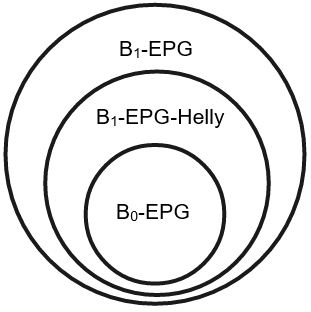
\includegraphics[width=3.5cm]{./img/diagramaClassesEPG.png}
\caption{Hierarchical diagram of some EPG classes}
\label{fig:diagramaEPG}
\end{figure}

In this section we describe representations of special graphs basis to our purposes. First, we consider EPG representations of $C_4$'s.

%By the results of \citep{golumbic2009}, in Lemma ~\ref{lem:representacaoC4}, every induced cycle of size 4 in a $ B_1$-EPG  representation  of $C_4$ has only a few possible representations.

\begin{defi} \label{defi:tortasFrame}

Let $ Q $ be a grid with a 4-star consisting of a point $b$ of $Q$,  and let $ (a_1, b),$ $(a_2, b),$ $(a_3, b),$ $(a_4, b)$ be edges of $ Q$ positioned as depicted at in Figure~\ref{fig:piesInGrid}(a). Let $ \mathcal{P} = \{P_1, \dots , P_4\}$ be a collection of paths each containing exactly two edges of the $4$-star:

\begin{itemize}
\item A \emph{true pie} is a representation where each $P_i$ of $ \mathcal{P} $ forms a bend in $b$.

\item A \emph {false pie} is a representation where two of the paths $P_i$ do not contain bends, while the remaining two do not share an edge. 

%In false pie only 2 paths not adjacent do bend in $b$.

\begin{figure}[htb]
  \centering
%segundo bloco de figuras
  \begin{tabular}{c c c c c }
    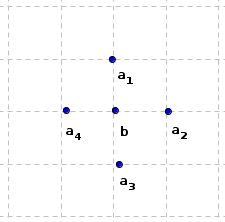
\includegraphics[width=4cm]{./img/disposicaoTortaGrid.png}    
    & &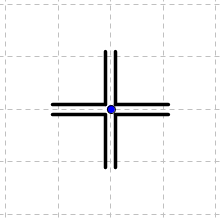
\includegraphics[width=4cm]{./img/truePieGrid.png} 
    & &
 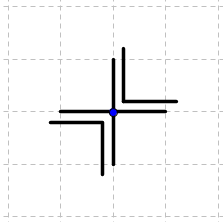
\includegraphics[width=4cm]{./img/falsePieGrid.png} \\%[\abovecaptionskip]
    {\footnotesize (a) 4-star in grid}  & &  {\footnotesize (b) True pie} & & {\footnotesize (c) False pie} %\label{fig:frame}
  \end{tabular}
  \caption{$B_{1}$-EPG representation of the induced cycle of size 4 as pies with emphasis in center $b$}\label{fig:piesInGrid}
\end{figure} 

\end{itemize}
\end{defi}
%In both cases the point $b$ is called \emph{center}, see Figures~\ref{fig:piesInGrid}(b) and~\ref{fig:piesInGrid}(c). There are edge-intersections $ (a_1, b), (a_2, b), (a_3, b), (a_4, b)$ called \emph{central rays}, see Figure~\ref{fig:piesInGrid}.

\begin{defi} \label{defi:tortasFrame2}
 Consider a rectangle of any size with 4 corners at vertices $ (x_1, y_1);$ $(x_2, y_1);$ $(x_2, y_2);$ $(x_1, y_2) $, positioned as in  Figure~\ref{fig:frameInGrid}. A \emph{frame} is a representation containing 4 paths $\mathcal{P} =  \{ P_1, \dots, P_4\} $, each having a bend in a different corner of a rectangle, and such that the  sub-paths $ P_1 \cap P_2, P_2 \cap P_3, P_3 \cap P_4, P_4 \cap P_1 $, share at least one edge. While the sub-paths $ P_2 \cap P_4 $ and $ P_1 \cap P_3 $ do not share edges.

\begin{figure}[htb]
  \centering
%segundo bloco de figuras
  \begin{tabular}{c c c c c }
    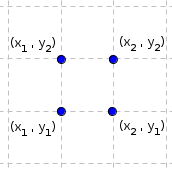
\includegraphics[width=4cm]{./img/dispositionFrameInGrid.png}    
    %& &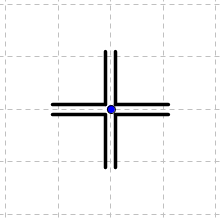
\includegraphics[width=4cm]{./img/truePieGrid.png} 
    & &
 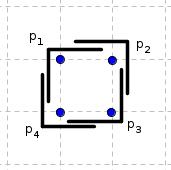
\includegraphics[width=4cm]{./img/frameInGrid.png} \\%[\abovecaptionskip]
    {\footnotesize (a) Points of the coordinates of bends of a frame}  
    %& &  {\footnotesize (b) True pie} 
    & & {\footnotesize (c) Paths of a frame} %\label{fig:frame}
  \end{tabular}
  \caption{$B_{1}$-EPG representation of the induced cycle of size 4 as frame}\label{fig:frameInGrid}
\end{figure} 

\end{defi}


%% \begin{figure}[htb]	
% \center%6.3
% 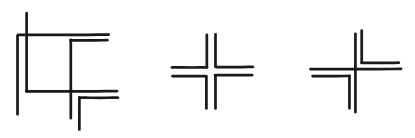
\includegraphics[width=10cm]{./img/representacaociclotam4.png}
% \caption{$B_{1}$-EPG representation of the induced cicle of size 4: frame (in left), true pie (center) and false pie (in right), \cite{golumbic2009}.}

% \end{figure}

\begin{figure}[htb]
  \centering
%segundo bloco de figuras
  \begin{tabular}{c c c c c }
    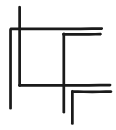
\includegraphics[width=2.3cm]{./img/representacaociclotam41.png}  
    & &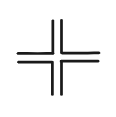
\includegraphics[width=2.5cm]{./img/representacaociclotam42.png} 
    & &
 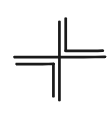
\includegraphics[width=2.5cm]{./img/representacaociclotam43.png} \\%[\abovecaptionskip]
    {\footnotesize (a) Frame}  & &  {\footnotesize (b) True pie} & & {\footnotesize (c) False pie} %\label{fig:frame}
  \end{tabular}
  \caption{$B_{1}$-EPG representation of the induced cycle of size 4}\label{fig:ciclotam4}
\end{figure} 


\begin{lema}\label{lem:representacaoC4}
\citep{golumbic2009} Every  $C_4$ that is an induced subgraph of a graph $ G $ corresponds, in any representation, to a true pie, false pie, or frame.
\end{lema}
% \begin{proof} Consider a collection of paths $ P = \ {P_1, \dots, P_4}$ of a grid $ Q $ in a $ B_1$-EPG representation of the graph $G$.

% Consider $ C_4 = (v_1, v_2, v_3, v_4) $ that is a chordless 4-cycle in $ G$. Consider $P_i$ the path in $ G $ that corresponds to $v_i $.
% Suppose $ \displaystyle \bigcap _{P_i \in P} P_i \neq \emptyset $, then clearly $ \displaystyle \bigcap _{P_i \in P} P_i = {b} $, for some point $ b $ of the grid. Since each vertex in $ C_4 $ has exactly 2 neighbors, each path $ P_i $ contains exactly two edges of the grid with end point $ b$. Thus, we obtain a star subgraph with center point $ b $ and edges $ (a_1, b), (a_2, b), (a_3, b), (a_4, b)$.
% Without loss of generality, $ P_1 $ contains the edges $ (a_1, b), (a_2, b) $ of the grid. If $ P_2 $ contains $ (a_2, b), (a_3, b) $ or $ (a_1, b), (a_4, b) $, then we get a true pie. Otherwise, $ P_2 $ contains the edges $ (a_2, b), (a_4, b) $ or $ (a_1, b), (a_3, b) $ and we obtain a false pie.

% Otherwise, $ \displaystyle \bigcaP_ {P_i \in P} P_i = \emptyset$. Suppose $ P_1 $ is a path without bend. Each of the $ P_2 $ and $ P_4 $ paths share an edge with $ P_1 $ but do not share a common edge with any other path. If $ P_2 $ and $ P_4 $ do not have a bend, then we get a interval representation of $ C_4 - v_3 $. However, it is not possible to add a $ P_3 $ path with at most of one bend. Similarly, if $ P_2 $ and $ P_4 $ have a single bend, the $ P_3 $ path can not be added either. Therefore, $ P_1 $ has a single bend.

% By symmetry, we assume that all $ P_i $ must has a single bend. Moreover, two paths can not have a bend on a common point in the grid. Thus, we obtain a rectangular subgraph with angles $ (x_1, y_1), (x_2, y_1), (x_2, y_2), (x_1, y_2) $, where $ P_1 $ bends at $ (x_1, y_1) $, $ P_2 $ bends at $ (x_2, y_1) $, $ P_3 $ bends at $ (x_2, y_2) $, and $ P_4 $ bends at $ (x_1, y_2) $, forming a frame.
% \end{proof}

\begin{defi}
%A edge is \emph{unnecessary} if its removal keeps the intersections and not intersection of the representation. 
A $B_k$-EPG representation is \emph{minimal} 
when its set of edges  is not properly contained in another $B_k$-EPG representation. 
%when all unnecessary edges are removed.
\end{defi}

An \textit{octahedral} is the graph containing 6 vertices and 12 edges, depicted  in Figure~\ref{fig:octaedro}(a). Next, we consider representations of the octahedral.

\begin{lema}\label{lem:octaedronaohelly}
The octahedral graph $O_3$ has a unique minimal  $ B_1$-EPG representation.%, without considering isomorphisms.
\end{lema}
\begin{proof}
The octahedral graph $ O_3 $ has in its constitution induced cycles of size 4 ($ C_4$'s). 
Take an induced $ C_4 $ subgraph  of the octahedral $ O_3 $. The pairs of non-adjacent vertices of the induced $C_4$ are false twins whose neighborhoods are the remaining of vertices of the induced $C_4$. Each of the vertices outside the $C_4$ are adjacent to all vertices of the $C_4$. Thus, if in a $ B_1$-EPG representation of $C_4$, the $ C_4 $ is represented as a frame, no single bend path can simultaneously intersect the 4 paths representing the vertices of the induced $ C_4 $. Therefore, we conclude that the frame structure can not be part of a $ O_3 $ representation.

With the same reasoning, take a $ B_1$-EPG representation of $C_4$ where the induced $ C_4 $ subgraph is represented as true pie or false pie. When adding the false twin vertices, which are neighbors of all vertices of $ C_4 $ taken from $ O_3 $, both representations converge to the structure represented in Figure~\ref{fig:octaedro}(b). 
\end{proof}

\begin{figure}[h]
  \centering
  
%segundo bloco de figuras
  \begin{tabular}{@{}c@{} p{1.5cm} @{}c@{} }
   \centering 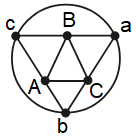
\includegraphics[width=3cm]{./img/octaedro.png} & &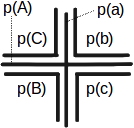
\includegraphics[width=3.5cm]{./img/representacaoOctaedro.png}  \\[\abovecaptionskip]
    \footnotesize \centering (a) The octahedral $O_3$ graph  & &  \footnotesize(b) $B_1$-EPG representation of the graph $O_3$
  \end{tabular}

 \caption{The octahedral $O_3$ graph and its  $B_1$-EPG representation}\label{fig:octaedro}
\end{figure}

By Lemma ~\ref{lem:octaedronaohelly},  $ O_3 $ has a unique minimal $B_1$-EPG representation, up to isomorphism, depicted in Figure~\ref{fig:octaedro}(b). The paths $ p(a), p(b) $ and $ p(c) $  do not satisfy the Helly property. Therefore $O_3 \notin B_1$-EPG-Helly. %From this observation and of the information shown in Lemma~\ref{lem:octaedronaohelly} we get the following. %Corollary~\ref{coro:b1hellyisinb1}.

% \begin{coro}\label{coro:b1hellyisinb1}
% %The x class is it's own subclass of the y class
% The $B_1$-EPG-Helly class is properly contained in the $B_1$-EPG class.
% \end{coro}

% \begin{lema}\label{lem:representationPolinomyal}
% For any $B_k$-EPG-Helly graph $G$ there exists  a $B_k$-EPG-Helly representation $Q$ of $G$ such that the size of $Q$ is bounded by $O(k+V(G))$.

% \end{lema}

% \begin{proof}

% Consider a minimal $B_k$-EPG representation of a graph $G$, with $n$ vertices, in which the largest coordinate used (on both the $x$ and $y$ axis) is normalized (first in $y$, and then in $x$, for example), and the smallest coordinate is $\geq 1$. Let $C$ be the value of the largest $x$-coordinate.

%  Therefore, all columns $1 \leq c \leq C$ are necessary for the representation, and correspond to the beginning, end, or bend of some path.

% The total number of starts, ends, and bends is n(k + 1), and at most $C \leq n(k + 1)$.

% %The reasoning can also be applied to vertical.
% \end{proof}


\section{Membership in $NP$}

%In this paper we are interested in characterizing the complexity of the $B_1$-EPG-Helly recognition problem, whose formal definition is presented next:
In this section, we show that the problem $B_k$-EPG-Helly recognition, where $k$ is bounded by a polynomial in $|V(G)|$, belongs to $NP$. The problem can be formally described as follows:


\begin{table}[h!]
\centering
%\caption{My caption}
%\label{my-label}
\begin{tabular}{ll}
\hline \hline
\multicolumn{2}{c}{\sc $B_k$-EPG-Helly Recognition}                                                                                                                                 \\ \hline \hline 
\emph{Input}: & A graph $G$.\\
~ & ~ \\
\emph{Goal:}  & \begin{tabular}[c]{@{}p{11cm}}
Determine if there is a set of single bend paths \\ $\mathcal{P} = \{P_1, P_2, \ldots, P_n\} $ in a grid $ Q $ 
such that:\\ 
$\bullet$ \ \ \ $u,v\in V(G)$ are adjacent in $G$ if only if $P_u,P_v$\\ \hspace{0.6cm} share an edge in $Q$; and\\
$\bullet$ \ \ \ $\mathcal{P}$ satisfies the Helly property.
\end{tabular} \\ \hline
\end{tabular}
\end{table}


A (positive) certificate for the {\sc $B_k$-EPG-Helly recognition} problem consists of a grid $Q$, a set $\mathcal{P}$ of single bend paths of $Q$, which have a one-to-one correspondence with the vertex set $V(G)$ of $G$, such that, for each pair of distinct paths $P_i, P_j\in \mathcal{P}, P_i\cap P_j \neq \emptyset $ if and only if the corresponding vertices are adjacent in $G$. Furthermore, $\mathcal{P}$ satisfies the Helly property.

% and a combining function $f$ that associates each vertex in a graph $G$ with a path  in $\mathcal{P}$ such that:

% \begin{itemize}
% \item for each $e=(u,v) \in E(G)$, it follows that $f(u)$ and $f(v)$ are intersecting in $Q$;
% \item for each $f(u),f(v) \in \mathcal{P}$ such that $f(u),f(v)$ are intersecting in $Q$, it follows that $(u,v) \in E(G)$;
% \item $\mathcal{P}$ satisfies the Helly property, i.e. every subset of paths pairwise intersecting in $\mathcal{P}$ has at least one common edge.
% \end{itemize}
% %\subsection{$B_k$-EPG-Helly is in NP}

The following concepts are central to our purposes. A \emph{relevant edge} in a  $B_k$-EPG representation is one which is either an extremity edge or a bend edge. Therefore each path with at the most $k$ bends can have $2(k+1)$ relevant edges, and any $B_k$-EPG representation contains at most $2|\mathcal{P}|(k+1)$ relevant edges.

The input for the verification algorithm of the certificate is a $B_k$-EPG representation $R$ containing a collection $\mathcal{P}$ of paths, $|\mathcal{P}|=|V(G)|$, where each path $P_i \in \mathcal{P}$ is given by its set of relevant edges plus the set of relevant edges of the paths that intersect $P_i$, the relevant edges are given in the order that they appear in the path. This coding format for the paths allow to verify if each set of relevant edges really represents a path in polynomial time.

In order to verify that the input, in fact is a certificate for the problem with size polynomial in $|V(G)|$, we have to assert the following:

\begin{enumerate}[label=(\roman*)]
\item The sequence of relevant edges of a path $P_i\in \mathcal{P}$ determines $P_i$ in polynomial time; \label{it:bullet1}

\item Two paths $P_i, P_j \in \mathcal{P}$ intersect if and only if they intersect in some relevant edge; \label{it:bullet2}

\item The set $\mathcal{P}$ of relevant edges satisfies the Helly property. The following lemma shows the above condition. \label{it:bullet3}
\end{enumerate}

\begin{lema}
Each path $P_i$ can be determined in polynomial time, from the considered sequence of edge.
\end{lema}

\begin{proof}
It is easy to verify that~\ref{it:bullet1} is true, consider the sequence of relevant edges of some path $P_i\in \mathcal{P}$. Start from an extremity edge of $P_i$. Let $t$ be the line (column) containing the last considered relevant edge. The next relevant edge $e'$ in the sequence, must be also contained in line (column) $t$. If $e'$ is an extremity edge, the process is finished and the path has been determined. It contains all edges between the considered relevant edges in the sequence. Otherwise, if $e'$ is a bend edge , the next relevant edge is the second bend edge $e''$ of this same bend, which is contained in some column (line) $t'$. The process continues until the second extremity edge of $P_i$ is located.   

With the above procedure, we can determine in $O(k+|V(G)|)$ time, whether path $P_i$ contains any given edge of the grid $Q$. Therefore, the sequence of relevant edges of $P_i$ uniquely determines $P_i$.
\end{proof}

The lemma below shows that~\ref{it:bullet2} holds.

\begin{lema}\label{lem:relevantEdges}
Let $R$ be a $B_k$-EPG-Helly representation of $G$, and $P_1, P_2 \in \mathcal{P}$ paths of $R$. Then $P_1, P_2$ are intersecting paths if and only if they contain a common relevant edge.
\end{lema}


\begin{proof}
If $P_1, P_2$ contain a common relevant edge there is nothing to prove. Otherwise, assume that $P_1, P_2$ are intersecting and we show they contain a common relevant edge. Without loss of generality, suppose $P_1, P_2$ intersect at line \textit{i} of the grid, in the  $B_k$-EPG representation $R$. The following are the possible cases that may occur:

\begin{itemize}
\item \textbf{Case 1:} Neither $P_1$ nor $P_2$ contain bends in line \textit{i}. 

Then $P_1$ and $ P_2$  are entirely contained in line \textit{i}. Since they intersect, either $P_1, P_2$  overlap, or one of the paths contains the other. In any these situations, they intersect in a common extremity edge, that is a relevant edge.

\item \textbf{Case 2:} $P_1$ does not contain bends in \textit{i}, but $ P_2$ does contain.

If some bend edge of $P_2$ also belongs to $P_1$, then $P_1, P_2$  intersect in  a relevant edge. Otherwise, since $P_1, P_2$  intersect, the only possibility is that the intersection contains an extremity edge of $P_1$ or $ P_2$. Hence the paths intersect in relevant edge.  

\item \textbf{Case 3:} Both $P_1$,  $P_2$ contain bends in \textit{i}

Again, if the intersection occurs in some bend edge of $P_1$  or $P_2$, the lemma follows. Otherwise, the same situation as above must occur, that is $P_1, P_2$  must intersect in same extremity edge.
 
\end{itemize}
In any of the cases, $P_1$ and $P_2$ intersect in some relevant edge.
\end{proof}

Finally, we prove~\ref{it:bullet3}.

% \begin{enumerate}[label=\roman*]
% \setcounter{enumi}{2}
% \item The set $\mathcal{P}$ of relevant edges satisfies the Helly property. The following lemma shows the above condition.
% \end{enumerate}

\begin{lema}
Let $\mathcal{P}$ be the set of relevant edges of a $B_k$-EPG representation $R$ of a graph $G$. We can verify that $R$ is Helly representation in polynomial time.
\end{lema}

\begin{proof}
Let $\mathcal{T}$ be the set of relevant edges of $R$. We consider each triple $T_i$ of edges of $\mathcal{T}$. Let $\mathcal{P}_i$ be the set of paths of $R$ containing at least two the relevant edges of $T_i$. If $R$ is a Helly representation, by Gilmore's theorem~\citep{bergeDuchet1975} the paths of $\mathcal{P}_i$  contain a common edge.  By Lemma~\ref{lem:relevantEdges} they contains a common relevant edge. Since there is a polynomial number of relevant edges, we can identify such a common edge, in polynomial time, and confirm that $R$ is in fact Helly. Since the number of triples is also polynomial, the lemmas follow.
\end{proof}

From (i), (ii) and (iii) we can then conclude.

\begin{theorem} \label{teo:npdificuldade}
A $B_k$-EPG representation of $G$ can be verified in polynomial time, for $k\leq |V(G)|^c$, for some fixed integer c.
\end{theorem}

%------------------------------
% Como, algoritmicamente ocorreria a identificacao de uma tripla de arestas não helly?
% perceba q da forma como estah, cada aresta relevante vai aparecer somente no caminho da qual ela faz parte, entao na situacao a seguir
%       e2 |
%   e1 ____ ____ e3
% De alguma forma tem que ser possivel verificar quais sao as interseccoes de cada aresta, ou entao colocalas em todo caminho que passa por ela. Pois sem essa informacao, nao eh possivel construir o certificado.
% ideia: manter uma lista de arestas de tamanho
% l = |P|*k+2k
% cada posicao representa uma aresta relevante da representacao e contem uma lista de todos os caminhos que passam por aquela aresta.

% pode existir um caminho x cuja uma aresta e' seja relevante para x mas não seja para y entao quando o algoritmo for pegar as triplas de caminhos que possuem no minimo duas arestas relevantes deixarah y de fora da computacao.

%------------------------------

% Consider that the number of bends $k$ of a $B_k$-EPG representation is polynomial with respect to the number of vertices $n$ of a graph $G$. If this occurs then the $B_k$-EPG representation has polynomial size, see Lemma~\ref{lem:representationPolinomyal}. 
% It is easy to check in polynomial time if all paths of a representation have at most $k$ bends. Thus, without loss of generality, the verification of the validity of a certificate for $B_k$-EPG-Helly recognizing just needs to compute in polynomial time if $ \mathcal{P} $ satisfies the  \textit{Helly property}. This result can be achieved through a generalization of Gilmore's Theorem \citep{bergeDuchet1975} which characterize $p$-Helly families. We consider $p=2$.

% Note that input datas to verify the validity of a certificate to YES are a $B_k$-EPG representation $R$ of a graph $G$ where $\mathcal{P}$ is the collection of paths that form $R$, each path $P_i \in \mathcal{P}$ is given by the set of coordinates of the relevant edges of $P_i$.

% \begin{lema}
% Let $R$ be a $B_k$-EPG representation of $G$, and $P_i,P_j$ paths of $R$ then if $P_i,P_j$ are intersecting paths they contain a common relevant edge.
% \end{lema}

% \begin{proof}
% If two paths $P_i$ and $P_j$ are intersecting paths then they share a edge of bend or they do not:
% \begin{itemize}
%     \item If they share a edge of bend  then this edge is a relevant edge;
%     \item If there is not edge of bend in the intersection $P_i$ and $P_j$ then the intersection $P_i$ and $P_j$ contains a path end that is a relevant edge of $P_i$ or of $P_j$.
% \end{itemize}
% \end{proof}

% \begin{theorem}
% A $B_k$-EPG Helly representation $R$ of $G$ can be recognizing in polynomial time.
% \end{theorem}

% \begin{proof}
% It follows that the number of relevant edges of $R$ is polynomial in $n$. Then we can verify that $R$ is a $B_k$-EPG representation in polynomial time. Next, we show that $R$ is really Helly.


% In addition, also replies that this is true for all triples of $\mathcal{T}$.

% Since the number of relevant edges is polynomial in $n$, this certificate can be verified in polynomial time.
% \end{proof}

\section{$NP$-hardness}\label{sec:sectionDispositivoClausula}

Now we will demonstrate that  $B_1$-EPG-Helly graph recognition is $NP$-complete. For this demonstration we set up a reduction from {\sc Positive (1 in 3)-3SAT} defined  as follows:

\begin{table}[h!]
\centering
%\caption{My caption}
%\label{my-label}
\begin{tabular}{ll}
\hline \hline
\multicolumn{2}{c}{\sc Positive (1 in 3)-3SAT}                                                                                                                                                                                                                                      \\ \hline \hline 
\emph{Input}: & \begin{tabular}[c]{@{}l@{}} a set $X$ of variables; a collection $C$ of clauses on $X$ where \\ for each $c\in C$, $c$ has only positive literal and $|c|= 3$.
\end{tabular} \\
~ & ~ \\
\emph{Goal:}  & \begin{tabular}[c]{@{}l@{}} 
Determine if there is an assignment of values to the variables \\in $ X $ so that every clause in $ C $ has exactly one true literal.
\end{tabular} \\ \hline
\end{tabular}
\end{table}

{\sc Positive (1 in 3)-3SAT } is a well known NP-complete problem (see \citep{johnson1979}, problem [L04], page 259). {\sc Positive (1 in 3)-3SAT} remains NP-complete when the incidence graph of the input CNF formula is a planar graph~\citep{mulzer2008minimum}.

Given a formula $F$ that is an instance of the {\sc Positive (1 in 3)-3SAT} we will present a polynomial-time construction of a graph $ G_F$ such that $ G_F $ is $ B_1$-EPG-Helly if and only if $ F $ is satisfiable. This graph will contain an induced subgraph $ G_c$ with 12 vertices (called \emph {clause gadget}) for every clause $ c \in C $, and an induced subgraph (\emph {variable gadget}) containing a particular vertex  $ v_j$ for every variable $ x_j$, plus a \emph{base gadget}  with 55 additional vertices.

%Since a Sun graph $S_4$ whose center is a cycle of size 4 and adding a false twin to each vertex of $S_4$ that is not a member of central induced cycle then we have the graph $H$. 
We will use a graph $H$ isomorphic to the graph presented in Figure~\ref{fig:gadgetBase}, as a gadget to perform the demonstration. For each clause $c$ of $F$ of the target problem, we will have a \emph{clause gadget} isomorphic to $H$, denoted by $G_c$. The graph $H$ consists of subgraphs whose $B_1$-EPG representations are well known, such as: cycles of sizes 3 and 4.

\begin{figure}[htb]	
\center%6.3
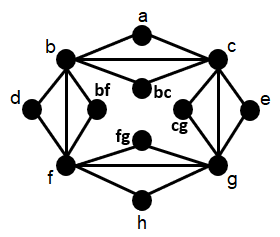
\includegraphics[width=4.5cm]{./img/gadgetBase.png}
\caption{The partial gadget graph $H$}
\label{fig:gadgetBase}
\end{figure} 

%\subsection{Definition}\label{sec:reducao}%The problem reduction}

The reduction of a formula $F$ from  {\sc Positive (1 in 3)-3SAT}  to a particular graph $G_F$ such that $G_F$ has a $B_{1}$-EPG-Helly representation if only if $F$ is satisfiable, it is given below.

\begin{defi}\label{sec:reducao}
Let $F$ be a CNF-formula with no negative literal, in which every clause has at most three literals. The graph $G_F$ is constructed as follows:

\begin{enumerate}
\item For each clause $C_i \in F$ create a  \textit{clause gadget} $G_{c}$, isomorphic to  graph $H$;%, that can be draw in single bend and Helly, as in same representation of the Figures~\ref{fig:falsepietruepieframe}(a), ~\ref{fig:falsepietruepieframe}(b) or~\ref{fig:falsepietruepieframe}(c)  ;

\item For each variable $x_{j}$ create a variable vertex $v_{j}$ that is adjacent to the vertex $a$, $e,$ or $h$ of $G_c$, when $x_{j}$ is the first, second or third variable in $C_i$, respectively;

\item For each vertex $v_{j}$, add two graphs  isomorphic to $H$, $H_1$ and $H_2$, where $v_{j}$ is  adjacent to all vertices of the triangle (a,b,c);%; (c,e,g); (g,f,h); or (b,d,f)) of each $H_1$ and $H_2$; 

\item The  subgraph induced by \emph{variable vertex}  $v_{j}$, and also $V(H_1)$ and $V(H_2)$ will be called \emph{variable gadget}; 

\item Create a vertex $V$, that will be used as vertical reference of the construction, and add edges from $V$ to each vertex  $d$;%$d \in V(G_c)$;

\item Create a bipartite graph $K_{2,4}$ with a particular vertex $T$ that is in the largest stable set. This vertex is nominated \emph{true vertex}. $T$ is adjacent to all $v_{j}$ and also to $V$;

\item Create two  graphs isomorphic to $H$, $G_{B1}$ and $G_{B2}$. The vertex $T$ is connected to all vertices of the triangle (a,b,c); %(c,e,g); (g,f,h); or (b,d,f)) 
of each one;


\item Create two isomorphic graphs at $H$, $G_{B3}$ and $G_{B4}$. The vertex $V$ is connected to all vertices of the triangle (a,b,c);% ((a,b,c); (c,e,g); (g,f,h); or (b,d,f)) of each;

\item The  subgraph induced by vertices $V(K_{2,4})$, $T$ and $V$,  $V(G_{B_1})$ and $V(G_{B_2})$, and also $V(G_{B_3})$ and $V(G_{B_4})$ will be nominated as \emph{base gadget}. 
\end{enumerate}
\end{defi}


The Figure~\ref{fig:exemploGrafoGF} represents the graph that would be obtained when the previous construction is applied to the formula $ F = (x_1 + x_2 + x_3) \wedge (x_2 + x_3 + x_4) \wedge (x_3 + x_1 + x_4)$.% $ on {\sc Positive (1 in 3)-3SAT}. %, the graph $ G_F $ will be like in the Figure~\ref{fig:exemploGrafoGF}.

%Consider that we can assign the following values to variables that will satisfy the formula $F$: $x_1 = False; x_2 = False; x_3 = True; x_4 = False$. Thus, considering this assignment we can have a $B_1$-EPG representation similar to the Figure~\ref{fig:grafoFormula}.


\begin{figure}[htb]	
\center%6.3
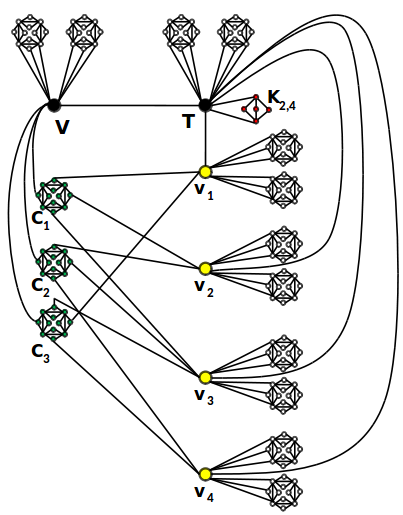
\includegraphics[width=8cm]{./img/exemploGrafoGFSBPO4.png}
\caption{The $G_{F}$ graph to formula $F=(x_1+ x_2+ x_3) \wedge  (x_2+ x_3+ x_4 )\wedge  (x_3 + x_1 + x_4 )$}
\label{fig:exemploGrafoGF}
\end{figure}

%\begin{figure}[htb]	
\center%6.3
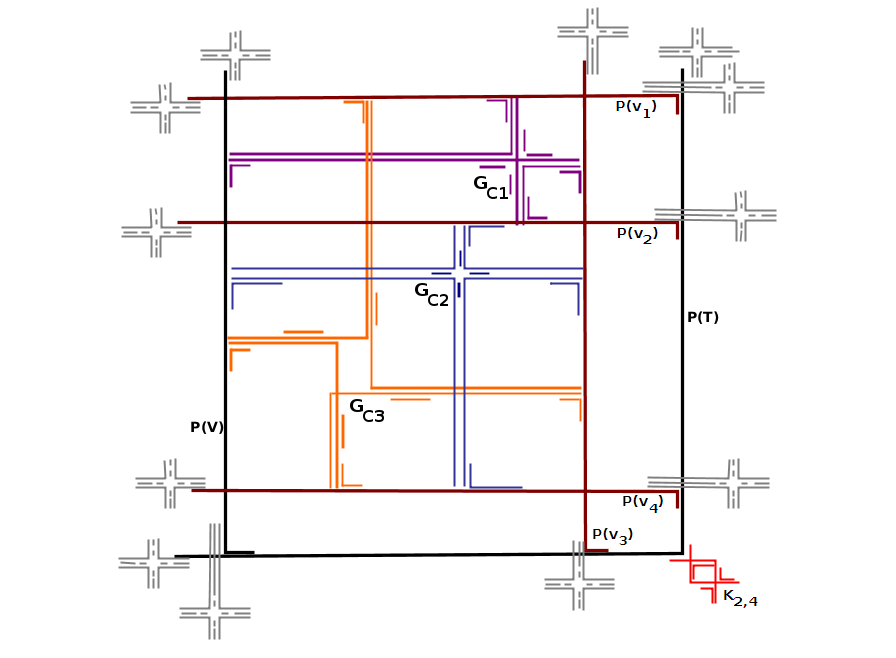
\includegraphics[width=1\textwidth]{./img/formulaGFCompletaSBPO3diferentes2.png}
\caption{The $B_{1}$-EPG-Helly representation to gadget $G_{F}$ of the Figure~\ref{fig:exemploGrafoGF}.%, to formula $F=(x_1+ x_2+ x_3) \wedge  (x_2+ x_3+ x_4 )\wedge  (x_1+ x_3+ x_4 )$. 
 The gadget's clause $G_{c_1}$ represented by false pie, the gadget's clause $G_{c_2}$ represented by true pie, and the gadget's clause $G_{c_3}$ represented by frame.}
\label{fig:grafoFormula}
\end{figure}


%First, we construct a minimal single bend representation for the base gadget, including the vertices $T$ and $V$. Such a representation, will be used as a base to guide as the representation of each clause gadget (i.e. $B_1$-EPG representation of $G_{c_i}$), is inserted in the structure. 

%\begin{figure}[htb]	
\center%6.3
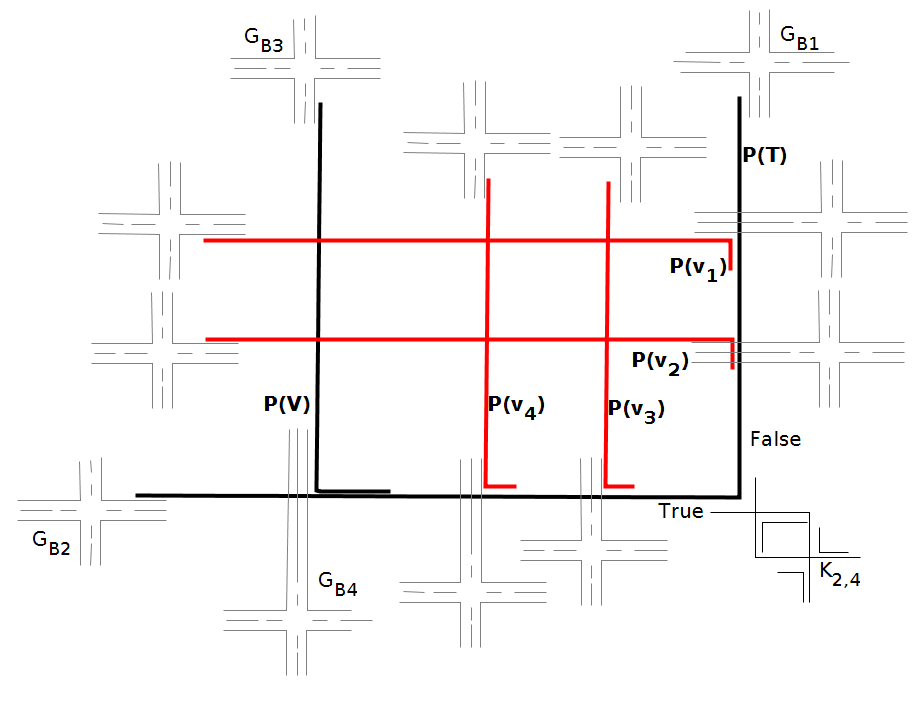
\includegraphics[width=10cm]{./img/gradeb1epghellySBPO.png}
\caption{Single bend and Helly representation of the forumla $F'$, no clause gadgets}
\label{fig:gradeb1epg}
\end{figure}

\begin{lema}\label{lem:ida}
Given a satisfiable instance $F$ of {\sc Positive (1 in 3)-3SAT}, the graph $G_F$ constructed from $F$ according to Definition~\ref{sec:reducao} admits a $B_{1}$-EPG-Helly representation.
\end{lema}

%Given an instance $F$ of {\sc Positive (1 in 3)-3SAT} we construct a graph $G_F$ as previously described. We will show that $G_F$ has a   $B_{1}$-EPG-Helly, $R_{G_F}$, representation if only if $F$ is satisfiable.


\begin{proof}

%~\ref{fig:representacaoCaminhos}
We will use the true pie and false pie structures to represent the \textit{clause gadgets} $ G_C$, but the construction could also be done with the frame structure without loss of generality, see Figure~\ref{fig:falseAndTruePie}.  


\begin{figure}[htb]
  \centering
%segundo bloco de figuras
  \begin{tabular}{c c c }
    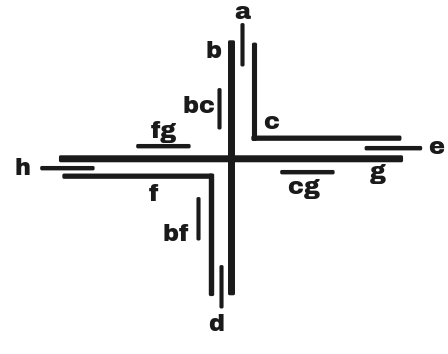
\includegraphics[width=6cm]{./img/falsePie.png}  %\label{fig:falsePie} 
    & &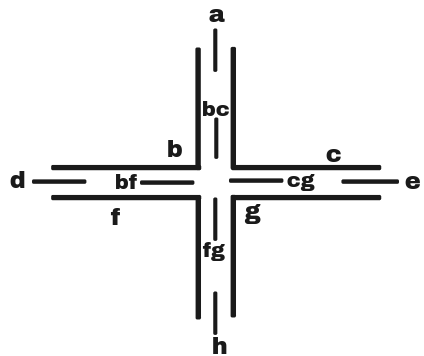
\includegraphics[width=6cm]{./img/truePie.png} %\label{fig:truePie}
    \\%[\abovecaptionskip]
    {\footnotesize (a) Based in false pie}  & &  {\footnotesize(b) Based in true pie}\\
  \end{tabular}
  \caption{Single bend representations of a clause gadget isomorph to graph $H$, see Figure~\ref{fig:gadgetBase}}\label{fig:falseAndTruePie}
\end{figure} 

The \textit{variable gadgets} will be represented by structures as of the Figure~\ref{fig:gadgetVariavel}.

\begin{figure}[htb]	
\center%6.3
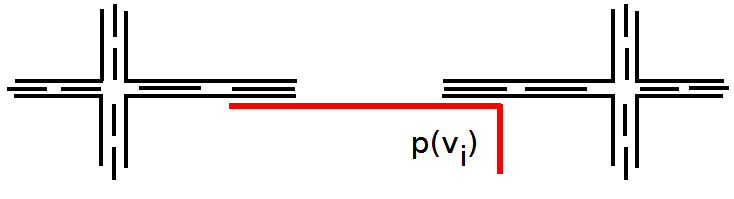
\includegraphics[width=10cm]{./img/gadgetVariavel.png}
%clausulaGadgetGFCompletaSBPO
\caption{Single bend representation of a variable gadget}
\label{fig:gadgetVariavel}
\end{figure}


The \textit{base gadget} will be represented by the structure of the Figure~\ref{fig:gadgetBaseSingleBend}.

\begin{figure}[htb]	
\center%6.3
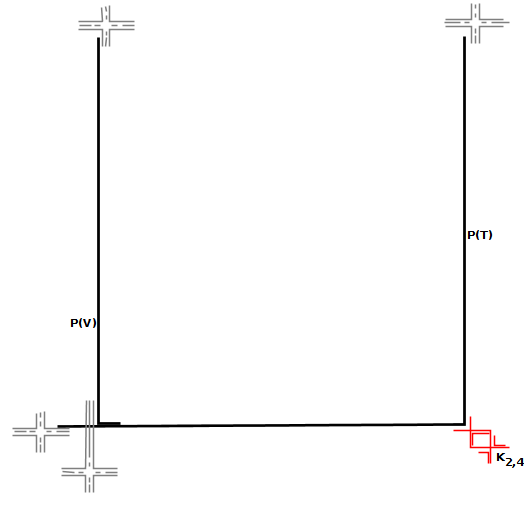
\includegraphics[width=10cm]{./img/gf2.png}
%clausulaGadgetGFCompletaSBPO
\caption{Single bend representation of the base gadget}
\label{fig:gadgetBaseSingleBend}
\end{figure}


It is easy to see that the representations of the clause gadgets, variable gadgets, and base gadgets are all $B_1$-EPG-Helly. Now we need to describe how these representations can be combined in order to construct a single bend representation $R_{G_F}$.

Given an assignment $A$ that satisfies $F$, we can construct a  $B_{1}$-EPG-Helly representation $R_{G_F}$. First we will fix the representation structure of the base gadget in the grid to guide the single bend representation, see Figure~\ref{fig:gadgetBaseSingleBend}. Next we will insert the variable gadgets with the following rule: if the  variable $x_i$ related to the path $p(v_i)$ had assignment \textit{True}, then the adjacency between the path $p(v_i)$ with $p(T)$ is horizontal, and vertical otherwise. For example, for an assignment $A=\{x_1=False; x_2=False;x_3=True; x_4=False\}$  to variables of the formula $F$ that generated the gadget $G_F$ of the Figure~\ref{fig:exemploGrafoGF}, it will give us a single bend representation (base gadget + variables gadget) according to the Figure~\ref{fig:gadgetBasePlusVariables}(a). 

 When a formula $F$ of {\sc Positive (1-in-3)-3sat} has clauses whose format of assignment is $(False, True, False)$ or $(False, False, True)$ then we will use false pie to represent these clauses, but when the clause has format $(True, False, False)$ we will use true pie to represent this clause. To insert a \textit{ clause gadget} $G_{C}$, we introduce a horizontal line $l_{h}$ in the grid between the horizontal lines used by the paths for the two false variables in $ C $. Then we connect the path $p(d_{c_i})$ of $G_{C_i}$ in $p(V)$ vertically using the bend of $p(d_{c_i})$. However, we introduce a vertical line $ l_{v}$ in the grid, between the vertical line of the grid used by $p(V)$ and the path to the true variable in $C_i$, i.e. between $p(V)$ and the path of the true variable $x_j \in C_i$. Where $l_{h}$ and $l_{v}$ cross, to insert the center of the  \textit{clause gadget} as can be seen in Figure~\ref{fig:gadgetOnePie}(b). A complete construction of this single bend representation for the $G_F$ can be verified in 
Figure~\ref{fig:gadgetFormulaCompletaPies}.%~\ref{fig:clausulagadgetgf}. 

\begin{landscape}
% \begin{figure}[htb]	
% \center%6.3
% 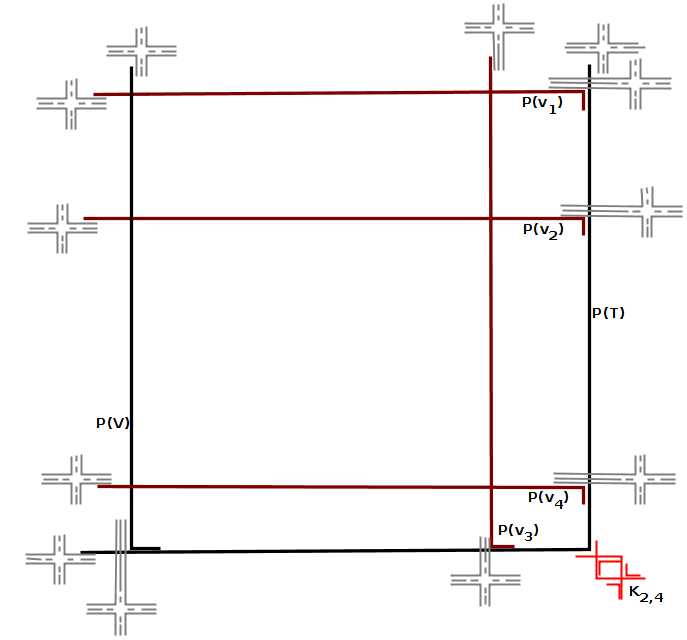
\includegraphics[width=10cm]{./img/gf3.png}
% %clausulaGadgetGFCompletaSBPO
% \caption{Single bend representation of the base and variables gadgets associated with the assignment $x_1=False, x_2=False, x_3=True, x_4=False$ }
% \label{fig:gadgetBasePlusVariables}
% \end{figure}
\begin{figure}[h]
  \centering
%segundo bloco de figuras
  \begin{tabular}{p{10cm} p{10cm}}
   \centering 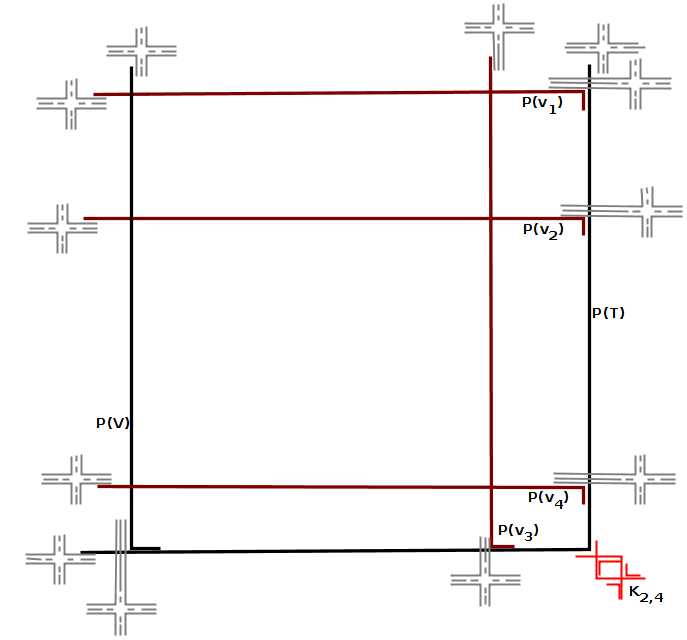
\includegraphics[width=10cm, left]{./img/gf3.png} & 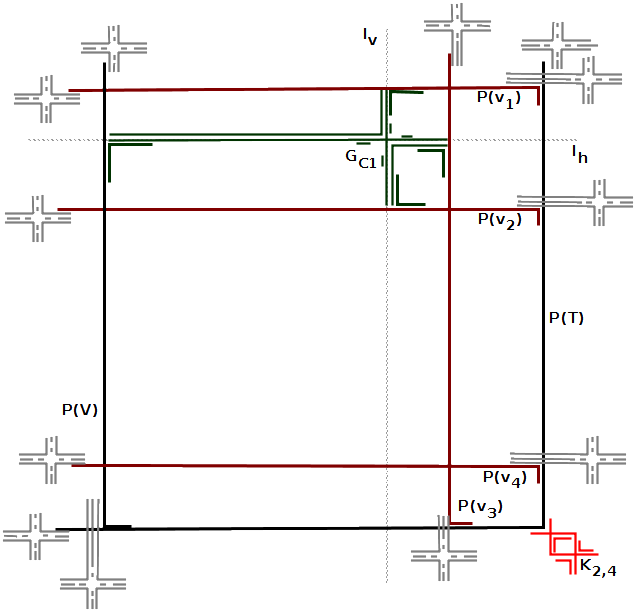
\includegraphics[width=10cm, left]{./img/formulaCompletaGFonePiePlusLines.png} \\  
  [\abovecaptionskip]
    \footnotesize \centering (a) Representation with omitted clause gadgets & \footnotesize(b) Representation with  $G_{C_1}$  associated with the clause $(x_1+x_2+x_3)$ in highlighted \\
%    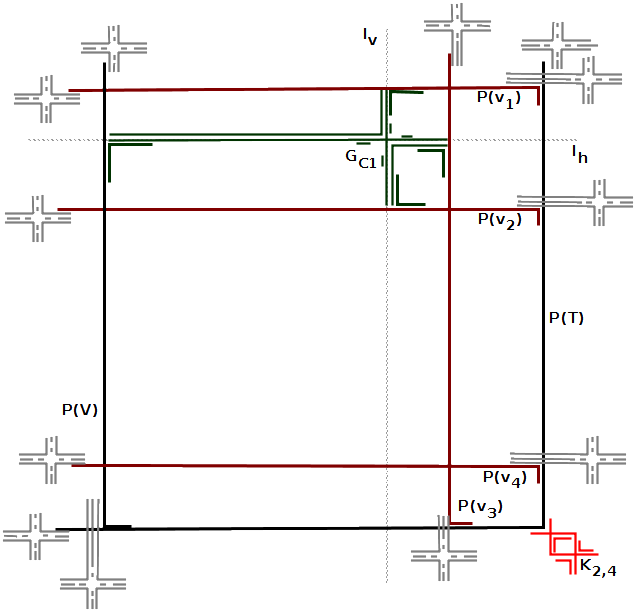
\includegraphics[width=10cm]{./img/formulaCompletaGFonePiePlusLines.png}
%   \\
%     \footnotesize(b) Representation with  $G_{C_1}$  associated with the clause $(x_1+x_2+x_3)$ in highlighted \label{fig:gadgetOnePie}
% \\
  \end{tabular}

 \caption{Single bend representation of the base and variables gadgets associated with the assignment $x_1=False, x_2=False, x_3=True, x_4=False$} \label{fig:gadgetOnePie} \label{fig:gadgetBasePlusVariables}
\end{figure}
\end{landscape}

%\begin{figure}[htb]	
\center%6.3
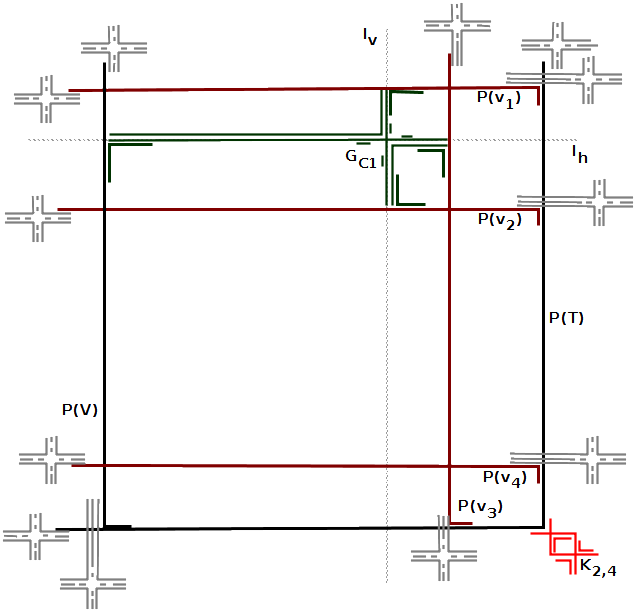
\includegraphics[width=10cm]{./img/formulaCompletaGFonePiePlusLines.png}
%clausulaGadgetGFCompletaSBPO
\caption{Single bend representation of the base and variables gadgets, and the clause gadget $G_{C_1}$  associated with the clause $(x_1+x_2+x_3)$ }
\label{fig:gadgetOnePie}
\end{figure}

\begin{figure}[htb]	
\center%6.3
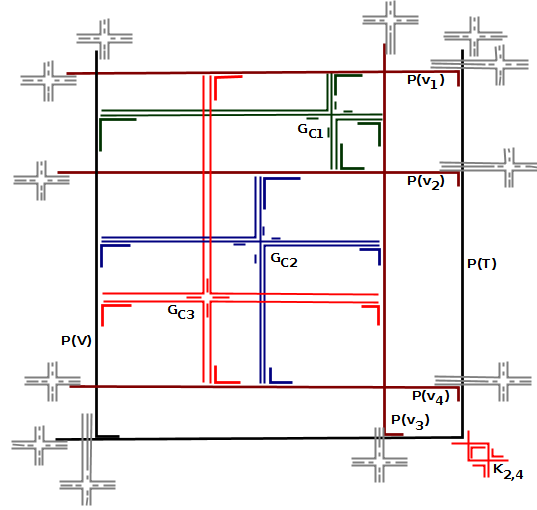
\includegraphics[width=10cm]{./img/formulaFGCompletaPies.png}
%clausulaGadgetGFCompletaSBPO
\caption{Single bend representation of $G_F$}
\label{fig:gadgetFormulaCompletaPies}
\end{figure}


% There is a permutation that we can represent all the settings for  $p(a_{c_i})$, $p(e_{c_i})$ e $p(h_{c_i})$, using pies, with $p(d_{c_i})$ fixed, these permutations are presented in the Figure~\ref{fig:disposicoes}. In other words,  it is possible to represent all combinations of assignments where the vertices $p(a_{c_i})$, $p(e_{c_i})$ and $p(h_{c_i})$ are relationship to variables with a assignment satisfiable. %Quando fixamos o $p(d)$, está ilustrado na 
% The Figure~\ref{fig:clausulagadgetgf} illustrates a provision for the relationship among the  $p(a_{c_i})$, $p(e_{c_i}), $ and $p(h_{c_i}) $, and variables with values $False$,  $True$, $False$, respectively.  

% \begin{figure}[h]
  \centering
  \begin{tabular}{ p{6cm} p{6cm} }
   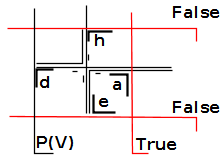
\includegraphics[width=6cm, left]{./img/clausulaGadgetDisposicoesefathf.png} & 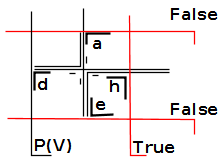
\includegraphics[width=6cm, left]{./img/clausulaGadgetDisposicoesefafht.png}
    \\
    \footnotesize \centering (a) $p(e), p(a), p(h)$ adjacent to variables with values $False, True,False$, respectively \label{fig:disposicao1} & \footnotesize(b) $p(e), p(a), p(h)$ adjacent to variables with values $False,False, True$, respectively \label{fig:disposicao2} \\
&  \\ 
  \end{tabular}

 \caption{Representation to differents variable arrangements, using structure of false pie.} \label{fig:disposicoes}
\end{figure} 

% \begin{figure}[htb]	
\center%6.3
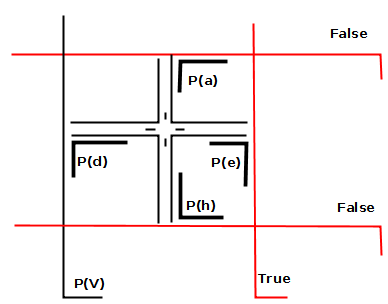
\includegraphics[width=8cm]{./img/falsepieInGrid.png}
%clausulaGadgetGFCompletaSBPO
\caption{Clause gadget positioned in a assignment satisfiable.}
\label{fig:clausulagadgetgf}
\end{figure}

Note that when we join all these representations of gadgets that form $ R_{G_F} $ we do not insert more bends in paths that had already bend then the representation is necessarily  $ B_1$-EPG. Let us show that it satisfies the Helly property. 

A simple way to check that $ R_{G_F} $ satisfies the Helly property  is to note that the particular graph $G_F$ never forms triangles between variable, clause, and base gadgets. Thus, any triangle of $G_F$ is inside a variable, clause or base gadget. As we only use $B_1$-EPG-Helly representations of such gadgets, $ R_{G_F} $ is a $B_1$-EPG-Helly representation of $G_F$.

% Another way to check is analyzing the representation, as we will do next.

% Let $\mathcal{P}_{1}$ be the set of paths of a clause gadget; let $\mathcal{P}_{2}$ be the set of paths of a variable gadget; and let $\mathcal{P}_{3}$ be the set of paths of a base gadget,  where each one of them are Helly and they are not intersecting, i.e. $\mathcal{P}_{1}\cap \mathcal{P}_{2} = \emptyset $, $\mathcal{P}_{2}\cap \mathcal{P}_{3} = \emptyset $, $\mathcal{P}_{3}\cap \mathcal{P}_{1} = \emptyset $, then $\mathcal{P}_{1}\cap \mathcal{P}_{2} \cap \mathcal{P}_{3} = \emptyset$. Take the set $\mathcal{P}_{3}$, for each variable gadget added to the drawing we are creating only one intersection between $P_i \cap P_j$ such that $P_i \in \mathcal{P}_{3}$ and $P_j \in \mathcal{P}_{2}$, therefore remains Helly.  

%Besides that to the insert the clause gadgets news intersections occur only between pairs of paths in distinct and independent sets from each other. Soon, the single bend representation remains Helly.
\end{proof}

%\cleardoublepage
%\newpage

To complete the prove of $NP$-hardness we will  present some considerations related with the single bend representation of gadgets that form the graph $G_F$. The way all gadgets can be drawn makes it possible to recover the formula that generated $G_F$ and a $True-$assignment for it. The following proofs help us understand the construction of a representation to $G_F$.  

%\subsection{Representations for the graph $C_4$}

\begin{defi}
Let $H$ be the graph shown in Figure~\ref{fig:gadgetBase} whose $H[\{b, c, f, g \}]$ in a single bend representation is by false pie or true pie, then:

\begin{itemize}
\item we denote by \emph{center} the unique grid-point of this representation in which is contained in every path representing the vertex in $ \{b, c, f, g \}$; \label{lab:lab1}

\item we denote by \emph {central ray} an edge-intersection  between two paths of $ \{b, c, f, g \} $ starting from the center.
\end{itemize}




% Let $H$ be the graph shown in Figure~\ref{fig:gadgetBase}. We denote by \emph{center} of a $B_1$-EPG representation of $H$ such that $H[\{b, c, f, g \}]$ is represented as false pie or true pie, the unique grid-point of this representation in which is contained in every path representing the vertex in $ \{b, c, f, g \}$.

\end{defi}

% \begin{defi}%\citep{golumbic2009}
% Let $H$ be the graph shown in Figure~\ref{fig:gadgetBase}. In each $B_1$-EPG representation of $H$, where $H[\{b, c, f, g \}]$ is represented as false pie or true pie, we denote by \emph {central ray} the edge-intersection  between two paths of $ \{b, c, f, g \} $ starting from the center.
% \end{defi}

Note that every $B_1$-EPG representation of a $C_4$ satisfies the Helly property, see Lemma~\ref{lem:representacaoC4}, and triangles have $B_1$-EPG representations that satisfy the Helly property, e.g. the one shown in Figure~\ref{fig:trianguloepgRepresentacao}(b). The graph $H$ is composed by a $C_4^{H}=H[b, c, f, g]$ and for eight cycles of size 3, which are $(a,b,c);$ $(b,c,bc);$ $(c,e,g);$ $(c,g,cg);$ $(f,g,h);$ $(f,g,fg);$ $(b,d,f);$ $(b,f,bf).$

As $C_4^{H}$ has a finite number of representations (see in Lemma~\ref{lem:representacaoC4}), then we can start drawing the $B_{1}$-EPG-Helly representation of $H$ from these structures.  Figures~\ref{fig:falsepietruepieframe}(a), ~\ref{fig:falsepietruepieframe}(b) and ~\ref{fig:falsepietruepieframe}(c) present 3 possible representations of $H$.

%The frame structure has characteristics different than the pies, which makes it less intuitive to understand, so we will make a more detailed discussion about the $B_1$-EPG representation of the frame structure to follow. %in Section~\ref{subsec:moldura}.

If $C_4^{H}$ is represented by pie, then the paths $p(b), p(c), p(f), p(g)$ share a central point of the representation, but if $C_4^{H}$ is represented by a frame then the bends of the 4 paths corresponding to the four distinct corners of a rectangle, i.e. all path representing a vertex of $C_4^{H}$ has a distinct bend point, see~\citep{golumbic2009}.

%As every vertex of $H$ has exactly two neighbors in $C_4^{H} $, then all paths in a $B_1$-EPG representation of $H$ are intersecting a pair of paths in the $B_1$-EPG representation of $C_4^{H}$. In this way, there will be exactly two paths that intersect each pair of central rays, see Figures~\ref{fig:falsepietruepieframe}(a) e~\ref{fig:falsepietruepieframe}(b). 

%\subsubsection{The special case of the frame structure} \label{subsec:moldura}

Due asymmetric representations, the frame structure needs to be studied in more detail. Next we will show some constraints of this structure. % in which allow us to consider it. %as gadget in the demonstration.

\begin{prop}\label{lem:direcoesdiferentes}
In a $B_1$-EPG representation of a $C_4$ isomorphic to a frame, every path $P_i$ that represents a vertex of the $C_4$ intersects exactly two other paths of the frame $P_{i-1}$ and $P_{i+1}$, so that one of the intersections is horizontal and the other is vertical. %where one of them is vertical and another is a horizontal intersection.
\end{prop}

\begin{proof}
The proof is immediate.
%Given a $B_1$-EPG representation of a $C_4$ isomorphic to a frame, where $P = \{P_1, \dots, P_4\}$ is the collection paths of this representation.  
%Every path has a bend with one part vertical and other horizontal. By contrary,  suppose there is a path $P_i$ of the frame $P = \{P_1, \dots, P_4\}$ both horizontally. Then we have that $P_i, P_{i-1}$ and $ P_{i + 1}$ have bend over the same straight line. But, by frame definition, these bend points should be the corners of a rectangle, a contradiction.
\end{proof}

\begin{prop}\label{lem:mesmaretasuporte}
Given a $B_1$-EPG-Helly representation of a graph $G$ that has an induced $C_4$ whose representation is isomorphic to a frame. If there is a vertex $v$ of $G$, outside this $C_4$, that is adjacent to exactly two consecutive vertices of this $C_4$, then the path representing $v$ shares at least one common edge-intersection with the paths representing both vertices.% of $v$ into such $C_4$.  
\end{prop}

\begin{proof}
%Consider $P_1$ and $P_2$ paths that represent consecutive vertices of the $C_4$, in a representation isomorphic at frame, and $B_1$-EPG-Helly such that $P_1 \cap P_2 \neq \emptyset$.
%Suppose that exist a third path, $P_x$, adjacent to $P_1$ and $P_2$, but $P_x \cap (P_1 \cap P_2) = \emptyset$. If this situation occurs, then the structure does not can be  Helly, a contradiction.
By assumption, $G$ has a triangle containing $v$ and two vertices of a $C_4$. Therefore the path representing $v$ shares at least one common edge-intersection with the paths representing these neighbors, otherwise the representation does not satisfy the Helly property.
\end{proof}

%\cleardoublepage

By Proposition~\ref{lem:direcoesdiferentes} and Proposition~\ref{lem:mesmaretasuporte} we can conclude that for every vertex $v_i \in V(H)$ such that $v_i \neq V(C_4^{H})$, when we use a frame to represent the $C_4^{H}$, $p(v_i)$ will have at least one common edge-intersection to a pair of paths equivalent to its neighbor vertices of $H$. %Then, in the Figure~\ref{fig:falsepietruepieframe}(a), Figure~\ref{fig:falsepietruepieframe}(b) and 
Figure~\ref{fig:falsepietruepieframe}(c) presents a possible $B_{1}$-EPG-Helly representation of $H$. On this $B_{1}$-EPG-Helly representation presented we can apply rotation and mirroring operations, because these operations do not change the structure. We can also a change the direction of the bend (see Figure~\ref{fig:falsepietruepieframe}(c) and Figure~\ref{fig:outraRepresentacaoFrame}), but also adjust other paths if needed, so as to not change the intersections between the paths.

\begin{defi}
In a single bend representation of a graph $C_4$ isomorphic to a frame, the paths that represent consecutive vertices in the $C_4$ are denoted by \emph{consecutive paths} and the segment that corresponds to the intersection between two consecutive paths is denoted \emph{side intersection}.  
\end{defi}

\begin{lema}\label{lem:2vertical2horizontal}
In any single bend minimal representation of a graph isomorphic to $H$, there are two paths in $\{p(a), p(e), p(d), p(h) \}$ that have horizontal direction and the other two paths have vertical direction.
\end{lema}

\begin{proof}
If the $C_4^{H} = [b,c,f,g]$ is  represented by a true pie or false then each path of $C_4^{H}$ share two central rays with two other paths of $C_4^{H}$, where each central rays corresponds to one pair of consecutive vertices in $C_4^{H}$.

As the vertices $a, e, d $ and $ h$ are adjacent to pairs of consecutive vertices in $C_4^{H}$ so the paths $p(a), p(e), p(d)$ and $p(h)$ have to be positioned in each one of the different central rays,  2 are horizontal  and 2 are vertical.

If the $C_4^{H}$ is  represented by a frame then each path of the $C_4^{H}$ has a bend positioned in  the corners of the frame. In the frame, the adjacency relationship of pairs of consecutive vertices in the $C_4^{H}$ is represented by the edge-intersection of the paths that constitute the frame. Thus, since a frame has two parts in the vertical direction and two parts in the horizontal direction, then there are two paths in $\{p(a), p(e), p(d), p(h)\}$ that have horizontal direction and two that have vertical direction.
\end{proof}

\begin{coro} \label{coro:paresMesmoSegmento}
In any single bend minimal representation of a graph isomorphic to $H$, the following paths are on the some central ray or side intersection: %have the some direction 

\begin{itemize}
\item $p(a)$ and $p(bc)$;
\item $p(e)$ and $p(cg)$;
\item $p(h)$ and $p(fg)$;
\item $p(d)$ and $p(bf)$.
\end{itemize}
\end{coro}

\begin{figure}[htb]
  \centering
%segundo bloco de figuras
  \begin{tabular}{c c c c c }
    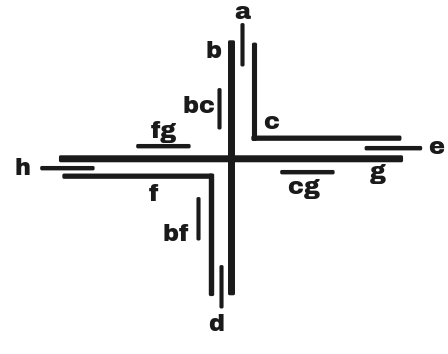
\includegraphics[width=4cm]{./img/falsePie.png}  %\label{fig:falsePie} 
    & &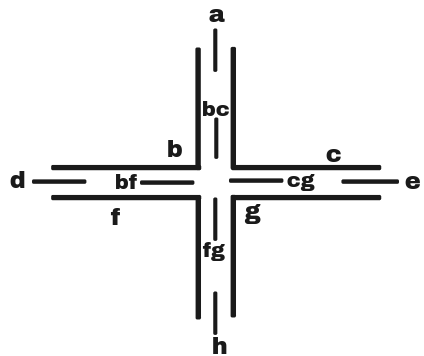
\includegraphics[width=4cm]{./img/truePie.png} %\label{fig:truePie}
    & &
 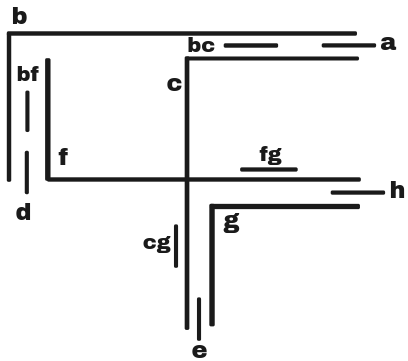
\includegraphics[width=4cm]{./img/frame.png} \\%[\abovecaptionskip]
    {\footnotesize (a) Based in false pie}  & &  {\footnotesize(b) Based in true pie} & & {\footnotesize (c) Based in frame} %\label{fig:frame}
  \end{tabular}
  \caption{Different single bend representations of the  graph $H$ using a false pie (a), a true pie (b) and a frame (c) for represent the $C_4^{H}$}\label{fig:falsepietruepieframe}
\end{figure} 

\begin{figure}[htb]	
\center%6.3
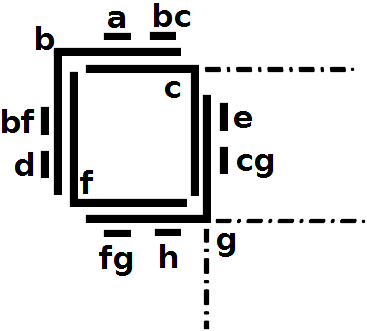
\includegraphics[width=4cm]{./img/outraRepresentacaoFrame.png}
\caption{Another frame representation, in dashed paths that have changed}
\label{fig:outraRepresentacaoFrame}
\end{figure}

\begin{defi}
Consider a graph $G$ and a vertex $v \in V(G)$. If in every $B_1$-EPG representation of $G$ the two bend edges (or one extremity edge) of the path $p(v)$ intersects other paths, then we say that $p(v)$ has an \emph{obstructed bend (or extremity)}. 
In addition, given a $B_1$-EPG representation of $G$ where $p(v)$ has an obstructed bend (or extremity), we say that a subset of paths \emph{obstructs} a bend edge (or a extremity edge) of $p(v)$ if it intersects such an edge. 


% Consider a single bend representation of a path $p$ with distinct edges-intersection with  $q$ and $q'$, both paths of the representation and not pairwise intersect. Thus a new path $p'$ added to representation such that $p'$ intersects $p$ and it does not intersect any $q$ and $q'$ then:

% \begin{itemize}
% \item  when $q$ intersects $p$ in an extremity edge and $q'$ intersects $p$ in another extremity edge then we have \emph{obstructed extremities} in $p$ for the path $p'$;
% \item  when $q$ intersects $p$ in an bend edge and $q'$ intersects $p$ in another bend edge then we have an \emph{obstructed bend} in $p$ for the path $p'$;
% \end{itemize}

%Consider a single bend representation of a path $p$ where one its extremities edges intersect one with $q$ and another with $q'$, both paths of the representation. Thus any new path $p'$ added to representation such that $p'$ intersects $p$ and it does not intersect any $q$ or $q'$  does not can intersect the extremities of $p$, when occur this situation then we have an \emph{obstructed extremity} in $p$. If bend edges of $p$ intersect one with $q$ and another with $q'$, both paths of the representation. Thus any new path $p'$ added to representation such that $p'$ intersects $p$ and it does not intersect any $q$ or $q'$  does not can intersect the extremities of $p$, then we say that there is a \emph{obstructed bend} in $p$.
\end{defi}


\begin{fact} \label{fact:k24facts}
In every single bend representation of a $K_{2,4}$, the path for each vertex of the larger part has its bend in a false pie (claim in~\citep{daniel2014b} and reasoning in~\citep{Asinowski2009}).
\end{fact}


\begin{lema}\label{lem:obstrucao}
In any single bend representation of the graph $G'$ presented in Figure~\ref{fig:extremidadeDobraObstruida}(a), the path $p(x)$ has obstructed extremities and bend.

%, i.e. another path $ p(q) $ can not be intersecting only the $ p(x) $ by the ends of the path nor by the bend.
\end{lema}

\begin{proof}
Consider $G'$ consisting of a vertex $x$, two graphs isomorphic to $H$, $ H_1 $ and $ H_2 $, and a bipartite graph $K_{2,4}$, such that: $x$ is a vertex of the largest stable set of the $K_{2,4}$; $x$ is adjacent to an induced cycle of size 3 of $H_1$, $C_3^{H_1}$ and to an induced cycle of size 3 of $H_2$, $ C_3^{H_2}$, see Figure~\ref{fig:extremidadeDobraObstruida}(a). %In any single bend representation of $G'$ the ends path and the bend of $p(x) $ are obstructed.

We know that the paths belonging to the largest stable set of a $K_{2,4}$ always will bend into a false pie, see Fact~\ref{fact:k24facts}. Since $p(x)$ is part of the largest stable set of the $K_{2,4}$, then $p(x)$ has an \emph {obstructed bend}, see Figure~\ref{fig:extremidadeDobraObstruida}(b). 

The vertex $x$ is adjacent to $ C_{3}^{H_1}$ and $ C_3^{H_2}$, so that its path $ p(x) $ intersects the paths representing them.  But in a single bend representations of a graph isomorph to $H$ there are pairs of paths that always are on some segment of a central ray or a side intersection, see Corollary~\ref{coro:paresMesmoSegmento}, and the representation of $C_{3}^{H_1}$ ( similarly $C_3^{H_2})$ has one these paths. Therefore, there is an edge in the set paths that represent ${H_1}$ ( similarly in ${H_2}$) that has a intersection of 3 paths representing $ C_{3}^{H_1}$ (and $ C_3^{H_2}$), otherwise the representation would not be Helly, and there is one other different edge in the some central ray or side intersection that contains three other paths and one of them is not in set paths  $C_{3}^{H_1}$ ( similarly $C_3^{H_2})$. Thus in a single bend representation of $G'$, the paths that represent  $C_{3}^{H_1}$ ( similarly $C_3^{H_2})$ must intersect in a bend edge or an extremity edge of $p(x)$, because $p(x)$ intersects only one of set paths that are on some central ray or side intersection where  $C_{3}^{H_1}$ ( similarly $C_3^{H_2})$ is. As the bend of $G'$ is already obstructed by structure of $K_{2,4}$, then ${H_1}$ ( similarly in ${H_2}$) must be positioned at an extremity edge of $p(x)$. This implies that $ p(x) $ has a condition of \emph{obstructed extremities}, see Figure~\ref{fig:extremidadeDobraObstruida}(b).


%So in each set paths representing ${H_1}$ and ${H_2}$, the path $ p(x) $ intersects only one

%them ($C_{3}^{H_1}$ and $ C_3^{H_2}$, precisely). 

%By Lemma~\ref{lem:2vertical2horizontal} follows that for any pair of paths $p', p''$ representing two vertices of the $C_4^{H}$, there are two pairwise non-intersecting paths that intersect both $p'$ and $p''$.

%Considering that only one of the two triples of vertices that share the same edge pair of $ C_4^{H} $ is adjacent to $ p(x) $, this implies that $ p(x) $ has a condition of \emph{obstructed extremities}, see Figure~\ref{fig:extremidadeDobraObstruida}.
%##############################
\end{proof}

\begin{figure}[h]
  \centering
  \begin{tabular}{p{6cm} p{1cm} p{6cm}}
     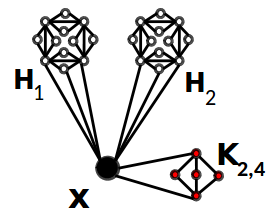
\includegraphics[width=5cm, center]{./img/grafoDobraExtremidadeObstruida.png} &  &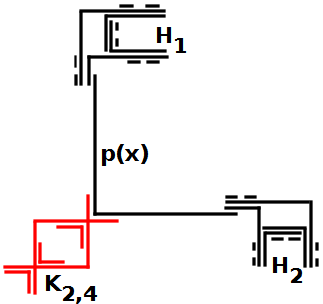
\includegraphics[width=5cm, center]{./img/extremidadeDobraObstruida2.png}  \\%[\abovecaptionskip]
    \footnotesize \centering (a) The graph $G'$& & \footnotesize \centering (b)A $B_1$-EPG representation of $G'$%\\
 %   &&
  \end{tabular}
 \caption{The sample of  obstructed extremities and bend.}\label{fig:extremidadeDobraObstruida}
\end{figure}

% -> Considere o grafo da Figura 9 (a), se adicionarmos um novo vertice y adjacente somente ao vertice x, então na B1-EPG representacao desse grafo o caminho p(y) possui um segmento maximal dominado por p(x). Isso significa que o segmento maximal de p(y) que é adjacente a p(x) estah totalmente contido em algum segmento de p(x), e ainda como p(x) possui dobra e extremidades obstruidas entao isso implica que o segmento maximal p(y) que eh adjacente a p(x) tambem estah obstruido.

% -> Duvida 1: inserir aqui tambem a parte que diz que se esse vertice y for adjacente a um outro vertice z entao obrigatoriamente y terah que possuir uma dobra?

% -> Duvida 2: Se a duvida anterior for incluida, entao posso incluir a situacao em que esse vertice y possui tambem suas mais dois elementos de obstrucao adjacentes a ele o que implica que alem do segmento maximal adjacente a p(x) tambem o segmento perpendicular (de dobra) tambem esta obstruido.  

%\begin{figure}[h]
  \centering
  \begin{tabular}{p{10cm} p{1cm} p{5cm}}
     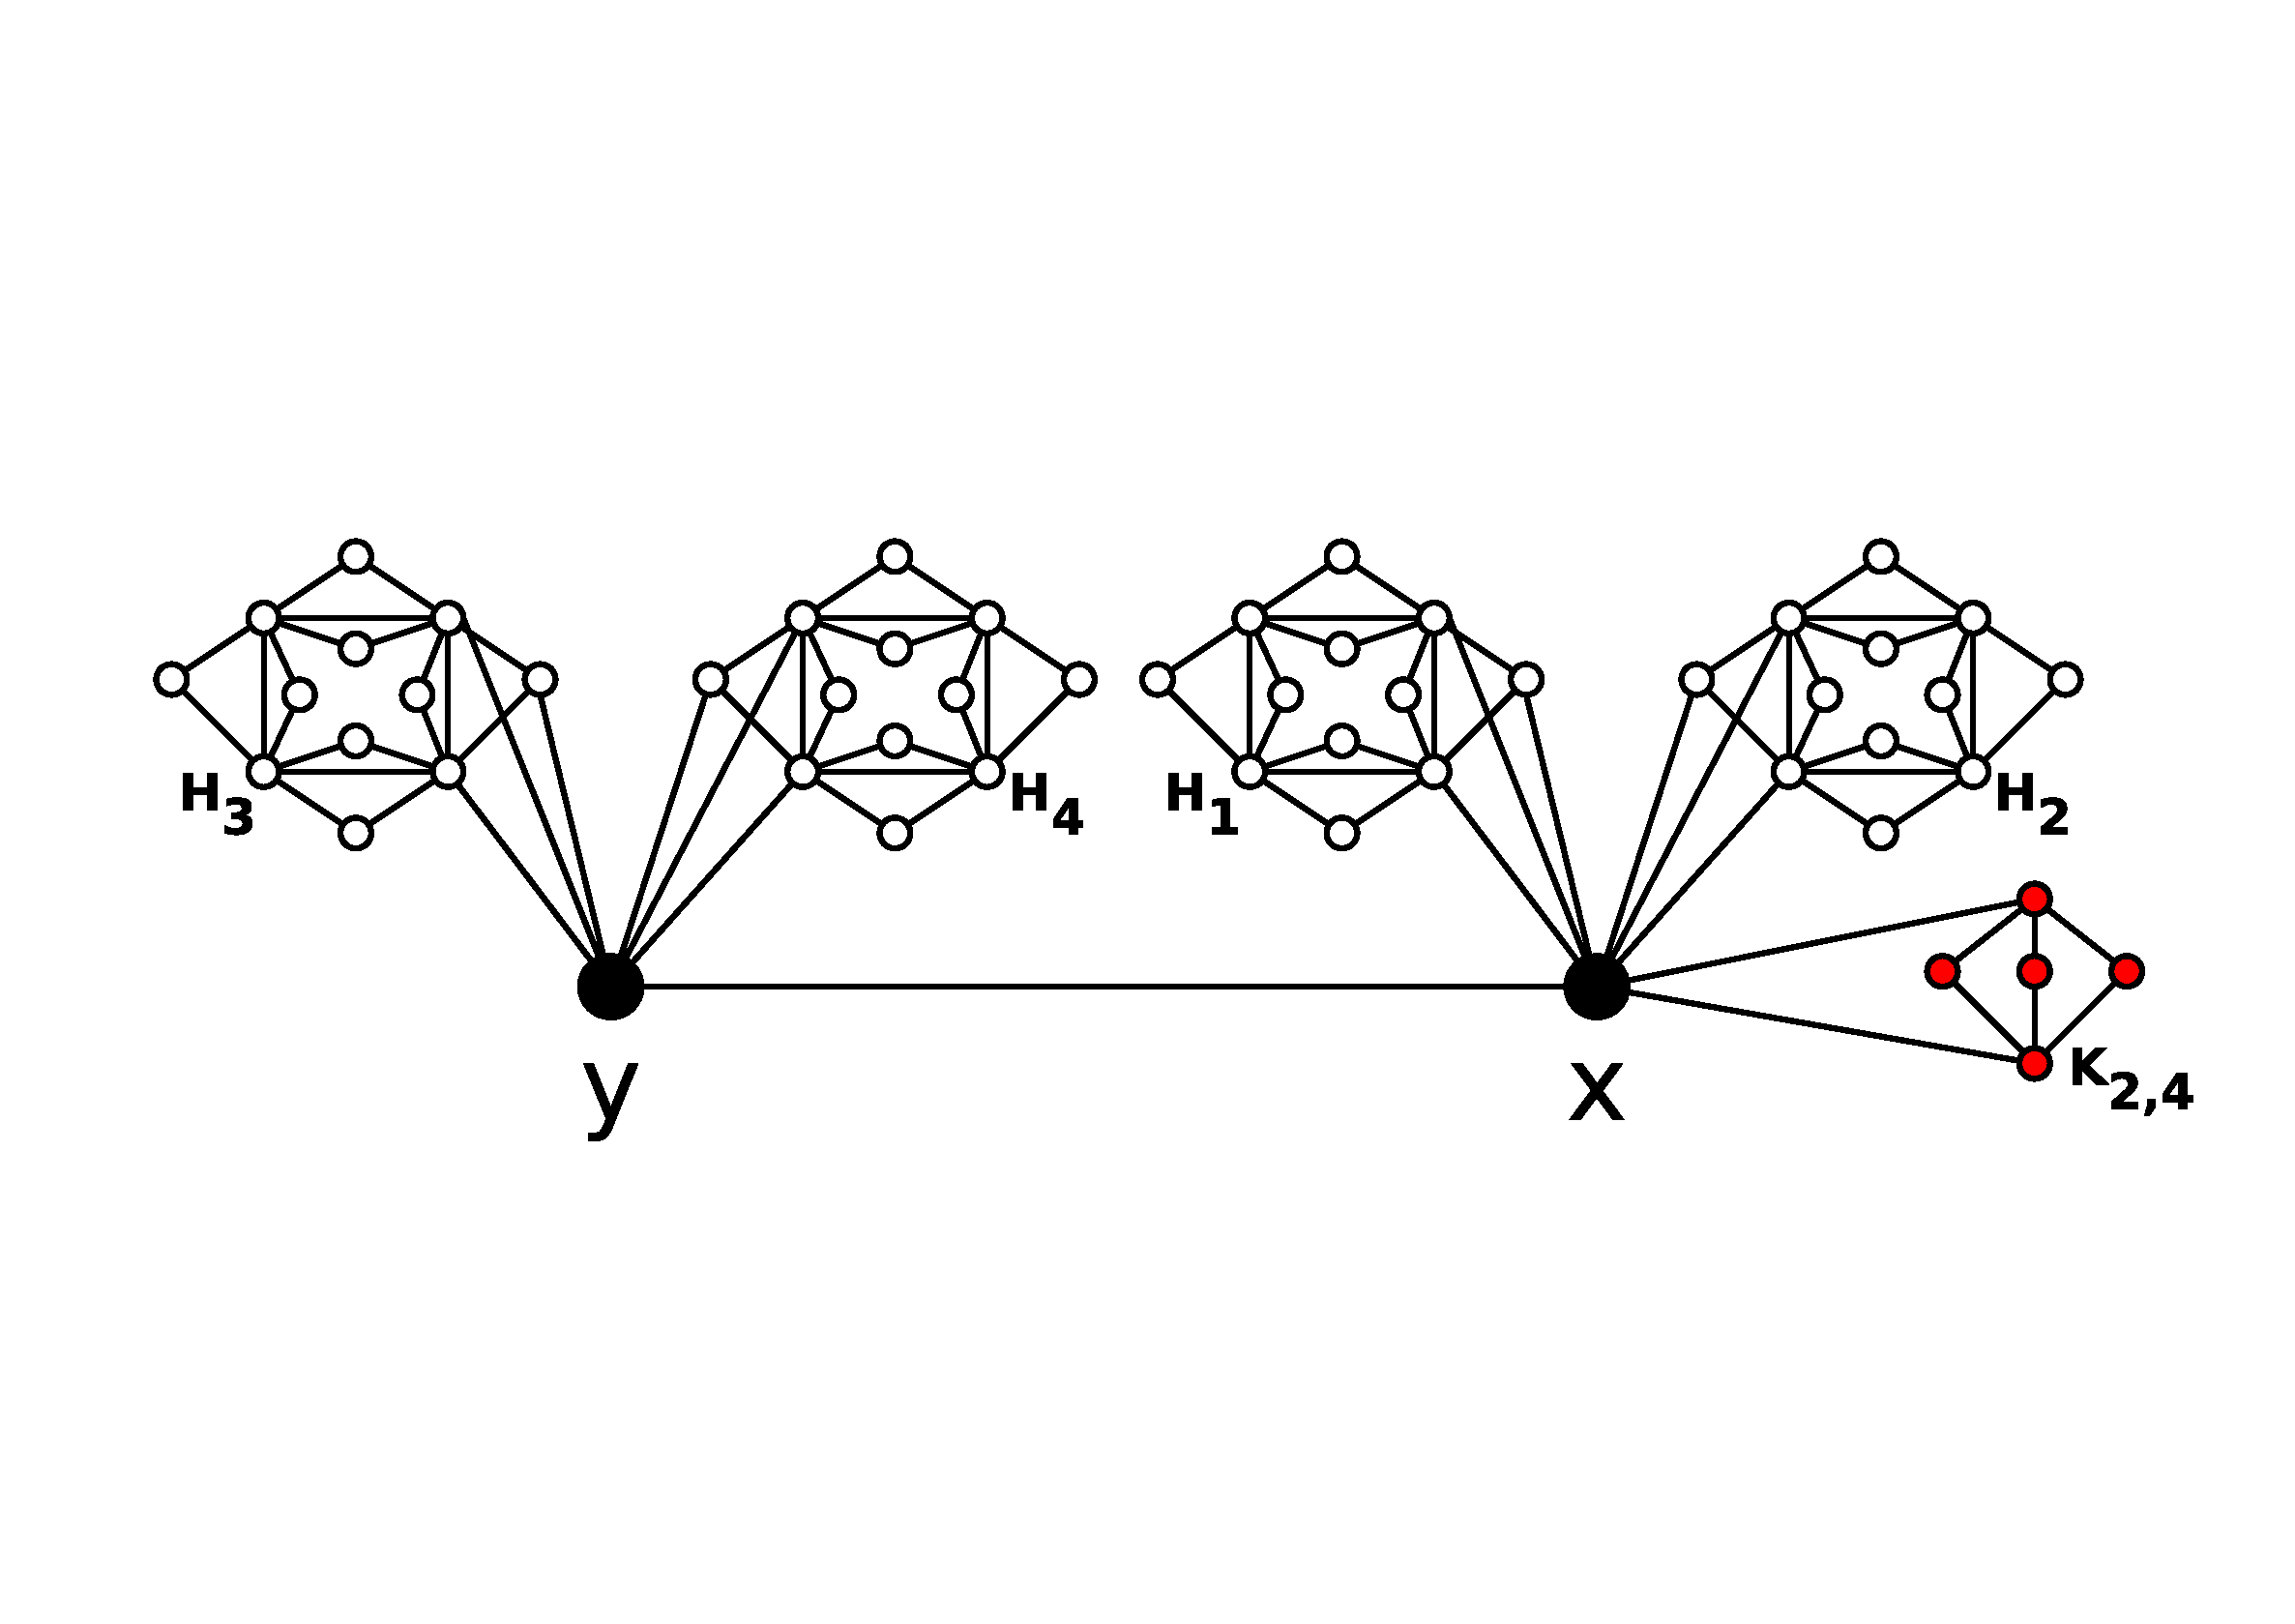
\includegraphics[width=10cm, center]{./img/obstrucaoDobraObstrucaoExtremidade2.eps} & &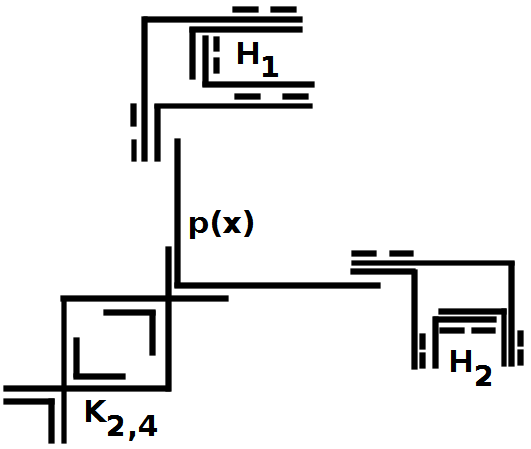
\includegraphics[width=5cm, center]{./img/extremidadeDobraObstruida.png}  \\%[\abovecaptionskip]
    \footnotesize \centering (a) The $G'$ graph& & \footnotesize \centering (b)A $B_1$-EPG representation of $G'$%\\
 %   &&
  \end{tabular}
 \caption{The sample of obstruction  end and obstruction bend}\label{fig:extremidadeDobraObstruida2}
\end{figure}



% \begin{lema}\label{lem:ida}
% Given a satisfiable instance $F$ of {\sc Positive (1 in 3)-3SAT} is possible to construct a gadget $G_F$ such that $G_F$ has a  $B_{1}$-EPG-Helly representation.
% \end{lema}

% %Given an instance $F$ of {\sc Positive (1 in 3)-3SAT} we construct a graph $G_F$ as previously described. We will show that $G_F$ has a   $B_{1}$-EPG-Helly, $R_{G_F}$, representation if only if $F$ is satisfiable.


% \begin{proof}
% Given an assignment that satisfies $F$, we can construct a  $B_{1}$-EPG-Helly representation $R_{G_F}$. First we represent every structure of the base gadget and the variable gadget, related to  $G_{F}$, with exception  \textit{clause gadgets},
% %@comment retirado para o SBPO
% %, como apresentado na Figura~\ref{fig:gradeb1epg}, 
% this construction must respect the restrictions presented in subsection~\ref{sec:reducao}. 


% Note that every single bend representation of a $K_{2,4}$ graph, the path of each vertex of the greater stable set, in particular $p(T)$ here represented, it has bend in a false pie, see \citep{Asinowski2009}. This condition forces $p(T)$ to bend in a false pie of any $B_1$-EPG representation of $K_{2,4}$. 

% The vertex $T$ is adjacent to vertices in a triangle of $G_{B1}$ and $G_{B2}$. As the $K_{2,4}$ is positioned in the bend of $p(T)$, thus in any $B_{1}$-EPG-Helly representation of $G_{B1}$  and of $G_{B2}$, they are positioned at the ends of $p(T)$, see Lemma~\ref{lem:obstrucao}.   

% A part of our \textit{base gadget} is isomorphic to graph $G'$ used in Lemma~\ref{lem:obstrucao} soon $p(T)$ has obstructed end and bend.  Without loss of generality assume that $p(V) \cap p(T)$ is a horizontal segment in  $R_{G_F}$.

% A path $p(v_{j})$ is connected to path $p(T)$ horizontally if $x_{j}$ is true and vertically otherwise. A part of each path $p(v_{j})$ is dominated by $p(T)$ and another part has obstructed end and bend by edge-intersection with a two triples of paths of $B_1$-EPG representation of graphs isomorphs to $H$.

% %~\ref{fig:representacaoCaminhos}
% Without loss of generality we will use the true pie and false pie structures to represent $ G_C$, but the construction could also be done with the frame structure (the Figure~\ref{fig:grafoFormula} presents the clause gadgets as false pie, true pie and frame).

% To insert a \textit{ clause gadget} $G_{C}$, we introduce an imaginary horizontal line $l_{h}$ in the grid between the horizontal lines used by the paths for the two false variables in $ C $. Then we connect the way $p(d_{c_i})$ of $G_{C}$ in $p(V)$ vertically using the bend of $p(d_{c_i})$. However, we introduce a vertical imaginary line $ l_{v}$ in the grid, between the vertical line of the grid used by $p(V)$ and the path to the true variable in $C_j$, i.e. between $p(V)$ and the path of the true variable $x_i \in C_j$. Where $l_{h}$ and $l_{v}$ cross, to insert the center of the  \textit{clause gadget} as can be seen in Figure~\ref{fig:clausulagadgetgf}. 

% There is a permutation that we can represent all the settings for  $p(a_{c_i})$, $p(e_{c_i})$ e $p(h_{c_i})$, using pies, with $p(d_{c_i})$ fixed, these permutations are presented in the Figure~\ref{fig:disposicoes}. In other words,  it is possible to represent all combinations of assignments where the vertices $p(a_{c_i})$, $p(e_{c_i})$ and $p(h_{c_i})$ are relationship to variables with a assignment satisfiable. %Quando fixamos o $p(d)$, está ilustrado na 
% The Figure~\ref{fig:clausulagadgetgf} illustrates a provision for the relationship among the  $p(a_{c_i})$, $p(e_{c_i}), $ and $p(h_{c_i}) $, and variables with values $False$,  $True$, $False$, respectively.  

% \begin{figure}[h]
  \centering
  \begin{tabular}{ p{6cm} p{6cm} }
   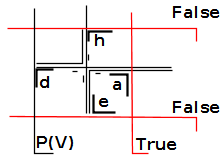
\includegraphics[width=6cm, left]{./img/clausulaGadgetDisposicoesefathf.png} & 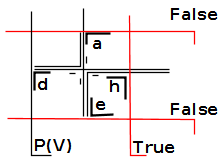
\includegraphics[width=6cm, left]{./img/clausulaGadgetDisposicoesefafht.png}
    \\
    \footnotesize \centering (a) $p(e), p(a), p(h)$ adjacent to variables with values $False, True,False$, respectively \label{fig:disposicao1} & \footnotesize(b) $p(e), p(a), p(h)$ adjacent to variables with values $False,False, True$, respectively \label{fig:disposicao2} \\
&  \\ 
  \end{tabular}

 \caption{Representation to differents variable arrangements, using structure of false pie.} \label{fig:disposicoes}
\end{figure} 

% \begin{figure}[htb]	
\center%6.3
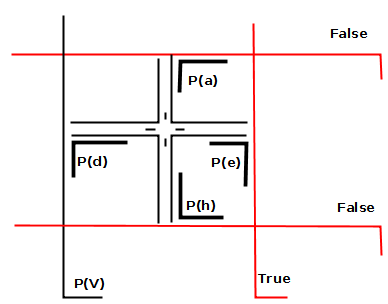
\includegraphics[width=8cm]{./img/falsepieInGrid.png}
%clausulaGadgetGFCompletaSBPO
\caption{Clause gadget positioned in a assignment satisfiable.}
\label{fig:clausulagadgetgf}
\end{figure}


% Note also that the single bend representation of the base gadget that we use respects the Helly property for the edges. Likewise, the single bend  representation of the clause gadget also respects the Helly property. Furthermore, the single bend representation of the set of vertices of the variable gadget respects the Helly property. And when we join all these representations of subgraphs in the graph of the formula $ G_F $, it also has a representation $ B_1$-EPG that respects the Helly property, when $ F $ is satisfiable.
% \end{proof}

\begin{defi}
We say that a segment $s$ is \emph{internally contained} into a path $p(x)$ if $s$ is contained into $p(x)$, and it does not intersect a relevant edge of $p(x)$. 
% In a single bend representation when there is a path $p(x)$ as in Figure~\ref{fig:extremidadeDobraObstruida}(b) that has obstructed bend and extremities, then a path $p(q)$ intersecting $p(x)$ but not intersecting the elements that obstruct $p(x)$ has a limitation to grow beyond the obstructions of $p(x)$, if this happens then $p(q)$ has \emph{segment dominated} by $p(x)$.
\end{defi}

\begin{fact}
In a single bend representation of a graph, if a path $p(y)$ has an obstructed bend and obstructed extremities, and some path $p(x)$ intersects $p(y)$, but does not intersect paths that obstruct the extremities and the bend edges of $p(y)$, then the intersection between $p(x)$ and $p(y)$ is internally contained into $p(y)$. 
\end{fact}


\begin{lema}\label{lem:volta}
If a graph $G_F$, construct according to Definition~\ref{sec:reducao}, admits a $B_1$-EPG-Helly representation, then the associated CNF-formula $F$ is a yes-instance of {\sc Positive (1 in 3)-3sat}.
\end{lema}

\begin{proof}
Suppose that $G_F$ has a $B_1$-EPG-Helly representation, $R_{G_F}$.  From $R_{G_F}$ we will construct an assignment that satisfies $F$. 

First, note that in every single bend representation of a $K_{2,4}$, the path of each vertex of the greater stable set, in particular $p(T)$ (in $R_{G_F}$), has bends contained in a false pie (see Fact~\ref{fact:k24facts}). %the explanation can be found in~\citet{Asinowski2009} apud~\citet{heldt2014}. This condition forces $p(T)$ to bend in a false pie of any $B_1$-EPG representation of $K_{2,4}$. 

The vertex $T$ is adjacent to the vertices of a triangle of $G_{B1}$ and $G_{B2}$. As the $K_{2,4}$ is positioned in the bend of $p(T)$, then in $R_{G_F}$ the representation of $G_{B1}$ and $G_{B2}$ are positioned at the extremities of $p(T)$, see Lemma~\ref{lem:obstrucao}.   

% A part of our \textit{base gadget} is isomorphic to graph $G'$ used in Lemma~\ref{lem:obstrucao} soon $p(T)$ has obstructed end and bend.  
Without loss of generality assume that $p(V) \cap p(T)$ is a horizontal segment in $R_{G_F}$.

We can note in $R_{G_F}$ that: the number of paths $p(d)$ with segment internally contained in $p(V)$ is the number of clauses in $F$; the intersection between each $p(a), p(e), p(h)$ in the gadget clause and each path $p(v_j)$ indicates the variables composing the clause. Thus, we can assign to each variable $ x_{j}$ the value \textit{True} if the edge intersecting $p(v_j)$ and $p(T)$ is horizontal, and \textit{False} otherwise. 


% A path $p(v_{j})$ is connected to path $p(T)$ horizontally if $x_{j}$ is true and vertically otherwise. A part of each path $p(v_{j})$ is dominated by $p(T)$ and another part has obstructed end and bend by edge-intersection with a two triples of paths of $B_1$-EPG representation of graphs isomorphs to $H$.


In Lemma~\ref{lem:2vertical2horizontal} it was shown that any minimal $B_1$-EPG representation of a clause gadget has two paths in $\{p(a), p(d), p(e), p(h)\}$ with vertical direction and the other two paths have horizontal direction. Since $p(d)$ intersects $p(V)$, it follows that in a single bend representation of $G_F$ we must connect two of these in order to represent a false assignment, and exactly one will represent a true assignment. Thus, from $R_{G_F}$ we construct an assignment to $F$ such that every clause has exactly one variable with a true value.  

%If a single bend Helly representation of the \textit{clause gadget} is isomorphic to the true or false pie, there are two paths that share same pair edge-intersection of a central ray. This block the clause gadget from positioning in an intermediate part of  $p(T)$, i.e. it has to be allocated in a end, explanation can be found in the section~\ref{sec:sectionDispositivoClausula}. 
% By Lemma~\ref{lem:mesmaretasuporte}, we know that if the base of the representation of the clause gadget it is a frame, a third vertex  adjacent to edge-intersection of a $C_4$ must share at least one these intersection segments. Thus, since there are two vertices in the \textit{clause gadget}  that share same neighborhood, at least one segment of each path of both vertices is on the same line support, which block the frame from having a completely contained side in a true vertex path $p(T)$. Thus, also in this case the clause gadget will be positioned at the end of the path of $p(T)$.

% As we take the adjacency between $p(V)$ and $p(T)$ horizontally, then any edge intersection in $p(V)$, with the exception of $p(T)$, obviously is vertical. Since $V$ is adjacent to vertices of the more external triangles in $G_{B3}$ and $G_{B4}$, the two vertical ends of the segments of $p(V)$ are obstructed by $G_{B3}$ and $G_{B4}$, respectively. Thus, the vertical segment of the path $p(d_{c_i})$ to each \textit{clause gadget} is completely contained in the vertical segment of $p(V)$.At that moment, the horizontal segments of each $p(d_{c_i})$, they must be positioned  to bending and to adjacency with $p(V)$. Consequently, if the $C_4^{H}$ of each clause gadget $G_c$ is  represented by a true pie or false so, the another three center ray, two are verticals and one is horizontal. If the $C_4^{H}$ of the \textit{clause gadget} $G_c$ is represented by a  \textit{frame},as frame has 4 distinct bends, where each path that is in $C_4^{H}$ is positioned in one of these bends, so always that $p(d_{c_i})$ is horizontal segment, also there will be two segments that are verticals and only one other path that is also horizontal (among $p(a_{c_i}),p(e_{c_i}), p(h_{c_i})$), otherwise the structure do not is a  \textit{frame}, see Lemma~\ref{lem:direcoesdiferentes}. The consequence of this structure, both for pies and frame is that this generates that in all \textit{clause gadget} the edege-intersection among only two $\{p(a_{c_i}), p(e_{c_i}), p(h_{c_i})\}$ and each $p(v_{j})$ are two horizontal and exactly one is vertical. In other words, every clause contains exactly one true variable.

% In any assignment the paths represented by $p(a_{c_i}), p(e_{c_i}), p(h_{c_i})$ have make bend to that there is intersection with $p(v_{j})$. Each \textit{variable gadget} has a pivot vertex  $p(v_{j})$ and two isomorphic graphs to $H$ with one more external triangle adjacent to $v_j$, as previously explained, these isomorphic graphs $H$, they must they can only connect at one end or bend of a path. Therefore, as the $p(v_{j})$ already does  adjacency with $p(T)$ then one of its ends is obstructed. It is then left to position the isomorphic to $H$ at the other end and in the bend of that path. In this way, any other vertex that is connected to   $p(v_{j})$ must connect in a do not extreme intermediate space. We conclude that $p(v_{j})$ is bend and end obstructed. 

% As the segments $p(a_{c_i}), p(e_{c_i}), p(h_{c_i})$ are two in vertical position and one  in horizontal position. Assuming $p(a_{c_i}), p(e_{c_i}), p(h_{c_i})$ can not connect to the paths of the variables by the ends, since these are already occupied. Whereas, furthermore,by Lemma~\ref{lem:mesmaretasuporte} and by definition of pies, $p(a_{c_i}), p(e_{c_i}), p(h_{c_i})$ do not can be completely contained in some $p(v_j)$ in the same direction as him. So necessarily, $p(a_{c_i}), p(e_{c_i}), p(h_{c_i})$ must connect to two paths of variables with false assignment (that connect vertically to
%  $p(T)$) and to a variable path with true assignment. Otherwise there would not be $R_{G_F}$.
%@comment os paragrafos acima estao sendo levados para proposicao 18 e lemma 19
\end{proof}

\begin{theorem}
{\sc $B_{1}$-EPG-Helly graph recognition} is NP-complete.
\end{theorem}
\begin{proof}
By Theorem~\ref{teo:npdificuldade} and Lemmas~\ref{lem:ida} and~\ref{lem:volta}.
\end{proof}

We say that a $k$-apex graph is a graph that can be made planar by the removal of $k$ vertices. In addition, a $d$-degenerate graph is a graph in which every subgraph has a vertex of degree at most $d$.

\begin{coro}
{\sc $B_{1}$-EPG-Helly graph recognition} remains NP-complete on $2$-apex and $3$-degenerate graphs.
\end{coro}
\begin{proof}

It is easy to see that the graphs constructed according to Definition~\ref{sec:reducao} are $3$-degenerate.
As {\sc Positive (1 in 3)-3SAT} remains NP-complete when the incidence graph of $F$ is planar~\cite{mulzer2008minimum}, from an instance $F$ of {\sc Planar Positive (1 in 3)-3SAT}, by using a planar embedding of the incidence graph of $F$, one can observe that by removing $V$ and $T$ from $G_F$ we obtain a planar graph. Thus, $G_F$ is 2-apex. 
\end{proof}




\section{References}
\bibliographystyle{elsarticle-num}
\bibliography{exemplo-latex}


\end{document}
\endinput
%%
%% End of file `elsarticle-template-num.tex'.
